\documentclass[a4paper,12pt,oneside]{scrartcl}
\providecommand{\chapterformat}{}
% Setup page
\usepackage[top=2.0cm, bottom=2.0cm, left=3cm, right=1.5cm, footskip=0.5cm]{geometry}
\usepackage{setspace}
\onehalfspacing
\usepackage[indent=1.0cm]{parskip}
\usepackage{epsfig}
\usepackage{xcolor}

% Base packages
\usepackage{fontspec}
\usepackage{booktabs}
\usepackage{xunicode}
\usepackage{xltxtra}
\usepackage{comment}
\usepackage{amsfonts}
\usepackage{amsmath}
\usepackage{longtable}
\usepackage{csquotes}
\usepackage{setspace}
\usepackage{placeins}
\usepackage{float}
\setcounter{tocdepth}{4}
\setcounter{secnumdepth}{4}
% Setup Russian hyphenation
\usepackage{polyglossia}
\setdefaultlanguage[spelling=modern]{russian} % for polyglossia
\setotherlanguage{english} % for polyglossia
\defaultfontfeatures{Scale=MatchLowercase, Mapping=tex-text}

% Setup fonts
\newfontfamily\russianfont{CMU Serif}
\newfontfamily\cyrillicfont{CMU Serif}
\setromanfont{CMU Serif}
\setsansfont{CMU Sans Serif}
\setmonofont{CMU Typewriter Text}


% Be able to include PNG and PDF as images
\usepackage{graphicx}
\usepackage{caption}
\usepackage{subcaption}

% Be able to insert hyperlinks
\usepackage{hyperref}
\hypersetup{colorlinks=true, linkcolor=black, filecolor=black, citecolor=black, urlcolor=black , pdfauthor=Zakharov Pavel <paltoszaharov@phystech.edu>, pdftitle=Диплом_бакалавриат}
\usepackage{url}

% Misc optional packages
\usepackage{footnpag}
\usepackage{indentfirst}
\usepackage{underscore}
\usepackage{amsthm}
\usepackage{enumitem} % continue enumeration 
\usepackage{mdwlist} % compact itemize lists environment
\usepackage{mdwlist} % compact itemize lists environment
%\renewcommand{\labelitemi}{--}  % Use endash for itemized lists
\usepackage[hang,flushmargin]{footmisc} % correct indent for footnotes


% Attach TikZ/PGF system to be able to draw vector plots.
% \usepackage{tikz}
% \usetikzlibrary{shapes, calc, arrows, fit, positioning, decorations, patterns, decorations.pathreplacing,chains, snakes}

% A new command to mark not done places
\newcommand{\todo}[1]{{\color{red}TODO\ #1}}
\onehalfspacing
\captionsetup[figure]{labelsep=endash, name=Рисунок, figurewithin=section}
\captionsetup[table]{margin=0cm, singlelinecheck=false, labelsep=endash, tablewithin=section}
\renewcommand{\thefigure}{\thesection.\arabic{figure}}
\begin{document}
\setcounter{page}{2}
%\begin{titlepage}
\thispagestyle{empty}

{\centering
Федеральное государственное автономное образовательное учреждение высшего образования 
<<Московский физико{}-технический институт (государственный университет)>>\par}

\bigskip
{\centering
Физтех-школа радиотехники и компьютерных технологий \par}

\bigskip
{\centering 
Кафедра микропроцессорных технологий в интеллектуальных системах управления
\par}

%\endhead

\bigskip

\bigskip


\vfill

{\centering\Large\bfseries
\textbf{Исследование мультиантенных систем в применении к беспроводным сенсорным сетям}
\par}

\bigskip

{\centering\bfseries
Выпускная квалификационная работа

(бакалаврская работа)

\bigskip
Направление подготовки: 03.03.01 Прикладные математика и физика
\par}

\vfill

\begin{tabular}{lll}\\
\specialcell{Выполнил:\\студент 516 группы}  & ______________ & Захаров Павел Сергеевич \\
                     &                &                  \\
Научный руководитель: & ______________ & Владимиров Леонид Леонидович \\
\end{tabular}

\vfill

{\centering
Москва 
2019
\par}

\end{titlepage}

\cleardoublepage

\begin{abstract}
В работе рассматриваются различные способы обработки сигналов с использованием нескольких антенн в применении к беспроводным сенсорным сетям.
Проведен обзор существующих технологий, использующих несколько антенных элементов.
Отобраны наиболее подходящие для использования в сенсорных сетях.
Проводится теоретическая оценка эффекта от их использования, определяются требования к оборудованию системы.
Кроме того, поставлены эксперименты, с помощью которых исследуется поведение этих методов на реальном оборудовании.
В случае восходящей линии связи подтверждена теоретическая производительность таких методов, как EGC и MRC.
Для нисходящей линии связи исследована чувствительность метода некогеретной передачи к временной синхронизации между антеннами. 
 
  
\end{abstract}
\clearpage

\tableofcontents
%\listoffigures
%\listoftables
\clearpage
\section{Список обозначений и сокращений}

\begin{table}[!htb]
\centering
\caption{Используемые обозначения и сокращения}
\label{designations}
    \begin{tabular}{|l|l|}
    \hline
    Обозначение & Значение \\ \hline
    WSN & Беспроводная сенсорная сеть \\
    SNR & Отношение сигнал-шум \\
    RSSI & Показатель уровня принимаемого сигнала \\
    PER & Уровень ошибок пакетов \\
    TX & Передатчик \\
    RX & Приемник \\
    MRC & Maximum Ratio Combining - \\
    & Объединение с максимальным отношением\\
    EGC & Equal Gain Combining -\\
    & Объединение с единичным усилением\\
    FSK & Частотная манипуляция \\
    SISO & Single-Input Single-Output\\
    $L$ & Длина пакета в отсчетах \\
    $l$ & Длина пакета в символах \\
    $h_i(\tau)$ & Импульсная характеристика канала между i-ой станцией и узлом\\
    $\alpha_i$ & Комплексное усиление канала между i-ой станцией и узлом\\
	$d(t)$ & Передаваемый сигнал \\	
	$s_i(t)$ & Сигнал на антенне i-ой базовой станции \\
	$s_{node}(t)$ & Сигнал на антенне узла \\
	$s_{base}(t)$ & Скомбинированный сигнал \\
	$n(t)$ & Шумовой сигнал \\
	$\Gamma_i$ & Отношение сигнал-шум на i-ой базовой станции \\
	$\Gamma_{node}$ & Отношение сигнал-шум на узле \\
	$\Gamma_{base}$ & Отношение сигнал-шум объединенного сигнала \\
    \hline
    \end{tabular}
\end{table}
\cleardoublepage

\section{Введение}
Развитие микроэлектроники произвело революцию в мире электронных устройств. 
На рынок вышли сотни новых видов электроники различного размера и назначения. 
В сочетании с развитием технологий передачи данных это привело к взрывному росту количества устройств, подключенных к сети Интернет. 
Так, к 2010 году это количество достигло 12.5 млрд при населении Земли в 6.8 млрд \cite{A1}. 
В этих условиях возникло понятие интернета вещей - глобальной инфраструктуры для информационного общества, которая обеспечивает возможность предоставления более сложных услуг путем соединения друг с другом (физических и виртуальных) вещей на основе существующих и развивающихся функционально совместимых информационно-коммуникационных технологий \cite{A2}.

%\begin{figure}[!htb]
%    \centering
%    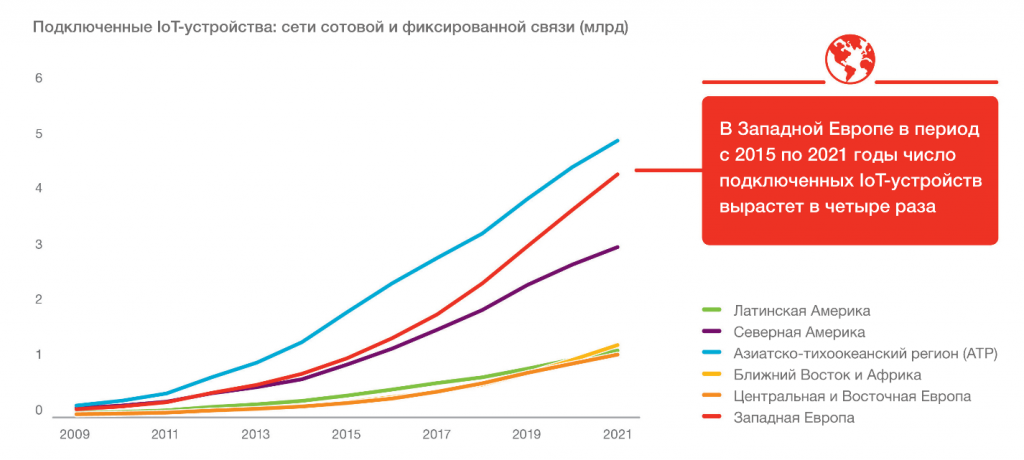
\includegraphics[width=0.9\textwidth]{pics/IoTgraph.png}
%    \caption{Типичная схема беспроводной сенсорной сети}
%    \label{fig:WSN}
%\end{figure}

Одной из ипостасей интернета вещей стали беспроводные сенсорные сети (Wireless Sensor Networks, или WSN), которые позволяют организовать автоматизированный сбор данных с больших территорий без необходимости разворачивать громоздкую инфраструктуру в виде кабелей передачи данных, проводов питания и т.д. 
Это качество делает их гибкими, простыми в разворачивании и дешевыми. 
В условиях появления у пользователей устройств, которые могут непосредственно взаимодействовать с сетью (смартфонов, планшетов и т.д.), и дальнейшего удешевления компонентов этих сетей WSN стали активно развиваться.

Сенсорные сети применяются в промышленности, жилищно-коммунальном хозяйстве, городской инфраструктуре, сельском хозяйстве, экологических и метеорологических исследованиях, системах охраны и многих других отраслях.


Такие сети, как правило, состоят из базовых станций, осуществляющих сбор данных с подчиненных им датчиков (узлов). 
Базовые станции далее обрабатывают полученные данные и посылают их на накопитель.
Сенсоры, однако, зачастую не могут использовать высокие мощности передатчика ввиду регуляторных ограничений и необходимости обеспечить как можно больший срок работы от батареи. 
Из-за этого установление радиоканала между датчиком и базовой станцией может быть затруднено. 
Для решения возникшей проблемы используются технологии ретрансляции и кооперации устройств, которые позволяют устройствам в сети объединяться для передачи данных \cite{B1}.

Обычно в подобных сетях одна базовая станция; соответственно, кооперируются обычно узлы сети. 
Однако в ряде случаев (офисные и жилые многоквартирные здания, промышленные предприятия) могут создаваться сети с несколькими базовыми станциями и соответствующими им сенсорами. 
Нередко эти базовые станции сами являются сенсором - к примеру, счетчиком электричества. 
При этом базовые станции могут быть связаны альтернативным каналом связи (PLC или традиционные кабели). 
Это позволяет использовать антенны базовых станций для связи с конкретным узлом, фактически выстраивая виртуальную мультиантенную систему. 
В таком случае могут использоваться соответствующие методы обработки сигналов. 
Тем не менее, в случае кооперативных методик антенны принадлежат разным устройствам, что создает дополнительные проблемы решения задач по синхронизации и обмену информацией. 

Еще одним обстоятельством является эволюционный подход к разработке систем. 
В случае, если комплекс разрабатывается не "с нуля", желательно максимально использовать уже существующие наработки и компоненты для упрощения поддержки и возможности модернизировать существующие реализации. 
Кроме того, необходимость поддерживать конкурентную стоимость разворачиваемой системы не допускает использование избыточно сложных и потому дорогих компонентов.

Таким образом, помимо вопроса относительно теоретической пользы использования подобных методов возникают задачи их применимости в сенсорных сетях в целом и в конкретной сети в частности.
Целью данной работы является нахождение наиболее подходящих для применения в беспроводных сенсорных сетях методов объединения пространственно разнесенных сигналов.
Для этого предлагается оценить теоретическую производительность методов, исследовать реальное поведение выбранных методов на моделях и прототипах, после чего на основании результатов работы оценить перспективы их использования с учетом существующей инфраструктуры.
\clearpage

\section{Обзор литературы}

Как указано выше, в данной работе исследуется кооперация базовых станций в WSN с целью улучшения качества сигнала.
На Рис.\ref{fig:GenScheme} показана схема исследуемой системы. 
Несколько базовых станций обмениваются данными со счетчиком, используя для взаимодействия альтернативный канал связи. 
Ради простоты и симметричности системы вычисления, связанные с обработкой принятых данных и подготовкой данных для передачи, выполняет выделенное устройство - точка обработки сигналов. 
Роль такой точки могут выполнять базовые станции, перидически меняющиеся между собой согласно определенному расписанию, либо же выделенное устройство.

\begin{figure}[!htb]
    \centering
    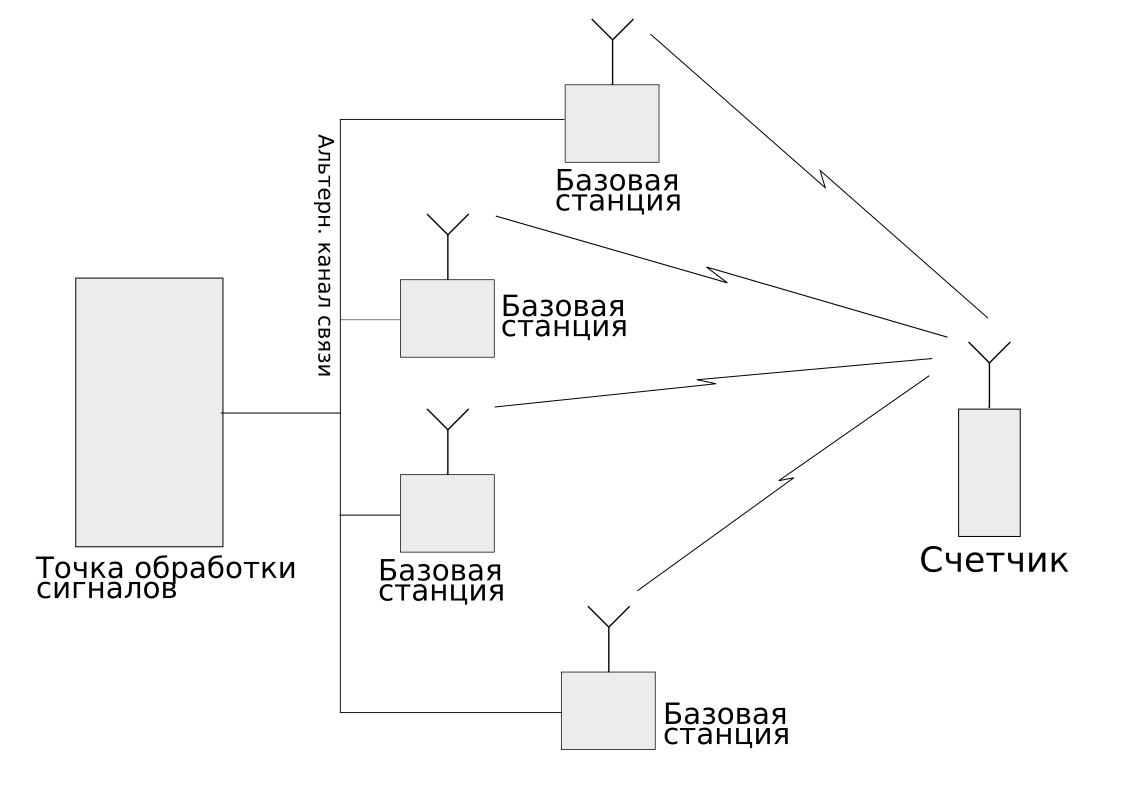
\includegraphics[width=0.9\textwidth]{pics/generalscheme.png}
    \caption{Общая схема предложенной системы}
    \label{fig:GenScheme}
\end{figure}

Стоит отметить, что восходящее (к базовым станциям) и нисходящее (к узлам) направления связи принципиально отличаются с точки зрения организации процесса передачи данных: в случае восходящей линии связи складываются низкочастотные оцифрованные сигналы внутри точки обработки сигналов, а в случае восходящей линии - радиочастотные на антенне. 
При этом все дополнительные вычисления происходят на базовых станциях в обоих случаях. По этой причине два направления будут рассмотрены отдельно.


\subsection{Восходящая линия связи}

При передаче данных на базовые станции приемники независимо друг от друга принимают и оцифровывают сигнал. 
Далее происходит обработка цифровых сигналов, их комбинирование. 
При этом изменения сигналов, возникающие из-за рассинхронизации принимающих антенн, можно считать особенностями каналов либо учесть и скомпенсировать в индивидуальном порядке. 
К примеру, фазовые сдвиги из-за различных осцилляторов и временные задержки из-за рассинхронизированных тактовых сигналов можно добавить к фазовым сдвигам и временным задержкам каналов, а частотные сдвиги нивелировать на каждой из станций, к примеру, с помощью пилот-сигналов\cite{A3}. 

Наиболее простыми в реализации являются алгоритмы, основанные на линейном комбинировании принятых сигналов. 
Такие алгоритмы преобразуют сигналы в цифровой области, что позволяет их реализовать на распределенной системе. 
По этой причине в данной работе внимание будет остановлено на них.
Выделяют две группы алгоритмов определения весов линейного комбинирования сигналов: алгоритмы пространственной и временной привязки \cite{B1}. 
Первые основываются на определении направлений прибывающих сигналов и выстраивании диаграммы направленности с тем, чтобы в указанных направлениях усиление было больше. 
Вторые основываются на применении пилотных сигналов. 
Используя их, алгоритм подбирает веса так, чтобы оптимизировать некоторую метрику качества приема, к примеру, SNR.
\subsubsection{Алгоритмы пространственной привязки}
Алгоритмы пространственной привязки, в свою очередь, также делятся на две группы. Первые используют геометрические параметры антенной решетки, вторые основываются на оптимизации тех или иных функционалов.

К первым относится, например, ESPRIT \cite{A4}, в котором предполагается, что решетка состоит из двух подрешеток, получающихся друг из друга параллельным переносом. 
Кроме того, можно упомянуть \cite{A5} и \cite{A6}. 
Первый предполагает линейную антенную решетку; второй не налагает требований на нее, но явно использует геометрическое расположение антенн.

Подобные требования тяжело удовлетворить на практике, т.к. фактическое расположение антенн зависит от здания, в котором разворачивается, количество и взаимное расположение базовых станций может существенно меняться от площадки к площадке. 
Более того, большинство подобных алгоритмов предполагают выполнение тех или иных моделей сигналов (к примеру, MUSIC и ESPRIT предполагают, что сигналы - плоские волны). 
Проверка применимости (и собственно применимость) моделей являются еще одной сложностью применения алгоритмов пространственной привязки. 
По этой причине они далее не рассматриваются в работе. 
\subsubsection{Алгоритмы временной привязки}
\begin{enumerate}
\item \textit{Сложение с единичным усилением (Equal Gain Combining - EGC)}. Предположим, что в канале равномерные медленные затухания:
\begin{equation}
h_i(\tau) = \delta(\tau)\alpha_i
\label{eq:impulse}
\end{equation} 
Тогда скомбинированный сигнал и SNR определяются следующими выражениями:
\begin{gather}
s_{base}(t) = \sum\limits_{i=1}^N \alpha_i^*s_i(t) \\
\Gamma_{base} = \sum\limits_{i=1}^N \Gamma_i
\label{eq:egc}
\end{gather}
\item \textit{Сложение с максимальным отношением (Maximum Ratio Combining - MRC)}. При том же предположении имеются следующие выражения для скомбинированного сигнала и его SNR:
\begin{gather}
s_{base}(t) = \sum\limits_{i=1}^N \frac{\alpha_i^*s_i(t)}{|\alpha_i|} \\
\Gamma_{base} = \frac{\left(\sum\limits_{i=1}^N \sqrt{\Gamma_i}\right)^2}{N}
\label{eq:mrc}
\end{gather}
\end{enumerate}
При равных отношениях сигнал-шум в каналах использование данных методов при $N=2$ может давать до 3 dB увеличения SNR, при $N=4$ - до 6 dB

\subsection{Нисходящая линия связи}
\subsubsection{Методы ретрансляции}
В случае нисходящей линии связи данные отправляются на узел. 
Так как узел имеет только одну антенну, малые вычислительные мощности и серьезные ограничения по энергопотреблению, то использовать комплексные методы обработки и демодулирования сигналов на принимающей стороне не представляется возможным. 
В этом случае используется ретрансляция:

Andreas F. Molisch в \cite{B1} приводит следующие основные практики ретрансляции:
\begin{enumerate}
\item \textit{Multi-hop}: последовательная пересылка данных от узла к узлу, пока информация не дойдет до пункта назначения. 
Является одним из наиболее популярных решений в беспроводных сенсорных сетях; тем не менее, в случаях, когда узлы находятся на больших расстояниях друг от друга, может возникать проблема обеспечения связности. 
Кроме того, на некоторые узлы может ложиться чрезмерная нагрузка по пересылке чужих пакетов.
\item \textit{Diversity} - сначала базовая станция рассылает данные всем доступным узлам (в т.ч. требуемому), затем  промежуточные узлы еще раз передают ту же информацию адресату.
\item \textit{Nonorthogonal Diversity} - передача конечному получателю одной и той же, но по-разному закодированной информации напрямую и через ретранслятор. 
В конечном итоге требуемый узел получает две версии полученной информации.
\item \textit{Intersymbol Interference} - Ретранслятор и источник информации передают данные со сдвигом в один символ. 
Пользователь получает по сути, данные с большими искусственно созданными межсимвольными помехами. В таком случае хорошо проявляют себя RAKE-приемники. \cite{A7}
\item \textit{Split-Combine} - рассылка данных доступным узлам, а затем коллективная одновременная передача на базовую станцию.
\end{enumerate}

В случае малошумящих входных трактов на узлах нередко происходит ситуация, когда отношение сигнал-шум достаточно высокое и позволяет демодулировать сигнал при условии обнаружения синхрослова. 
Сигнал при этом очень сильно ослаблен, и потому узел просто не может заметить, что ему что-то передают. 
С помощью Split-Combine можно увеличить мощность сигнала и таким образом получить лучшие результаты на границе области приема. 
По этой причине в работе рассматриваются методы именно типа Split-Combine. 
Intersymbol Interference алгоритмы также позволяют накапливать мощность от компонент, однако существенно повышают сложность реализации узла.

По аналогии с методами объединения для восходящей линии связи можно отметить два варианта предобработки сигналов, предназначенных на передачу:

\begin{enumerate}
\item \textit{Передача с максимальным отношением} является аналогом сложения с максимальным отношением. Пусть $h_i\left(\tau\right)=\alpha_i\delta\left(\tau\right)$ - импульсные характеристики каналов от антенн передачи на антенну приема, $d\left(t\right)$ - сигнал, который требуется передать. 
Тогда, если i-ая антенна передает сигнал $s_i\left(t\right) = A\alpha^*_id\left(t\right)$ 
\newline ($A$ - некоторая константа, компенсирующая малость $|\alpha_i|$. К примеру, $A = \frac{1}{min\{|a_i|\} }$), то принятый сигнал имеет вид:
\begin{equation}
s_{node}\left(t\right)=\sum\limits_{i=1}^N A\alpha_i\alpha^*_id\left(t\right) + n\left(t\right) = A\left(\sum\limits_{i=1}^N |\alpha_i|^2\right)d\left(t\right) + n\left(t\right)
\end{equation} 
\item \textit{Передача с единичными усилениями}, в свою очередь, является аналогом сложения с единичными усилениями. 
При тех же предположениях на импульсные характеристики каналов i-ая антенна передает сигнал i-ая антенна передает сигнал $s_i\left(t\right) = \frac{\alpha^*_i}{|\alpha_i|}d\left(t\right)$, то принятый сигнал имеет вид:
\begin{equation}
s_{node}\left(t\right)=\sum\limits_{i=1}^N \alpha_i\frac{\alpha^*_i}{|\alpha_i|}d\left(t\right) + n\left(t\right) = \left(\sum\limits_{i=1}^N |\alpha_i|\right)d\left(t\right) + n\left(t\right)
\label{eq:egtsignal}
\end{equation}
\end{enumerate}
Передача с единичным усилением не требует знания усиления в канале, в отличие от предыдущего метода. Нужно знать только фазовые сдвиги.  

\clearpage

\section{Постановка задачи}

В предыдущем разделе были описаны основные варианты применения пространственно разнесенных сигналов. Некоторые из них уже были по тем или иным причинам отмечены, как неподходящие/неинтересующие. Оставшиеся, тем не менее, требуют дальнейшего рассмотрения. 
Для каждого из них требуется провести следующие изыскания:
\begin{enumerate}
\item Провести теоретическую оценку производительности метода в терминах метрик качества сигнала (либо провести моделирование системы);
\item Оценить возможность реализации алгоритма, определить или уточнить требования к каналу, оборудованию, алгоритмам обработки данных;
\item Реализовать экспериментальную установку - модель системы с реализованным методом;
\item Провести эксперименты с моделью, уточнить требования к реальной системе, возможность их удовлетворения, сопоставить теоретические результаты с экспериментальными;
\item Определить возможности для модернизации метода.
\end{enumerate}

\clearpage

\section{Экспериментальная установка}
Общая схема экспериментальной установки, используемой для проведения экспериментов показана на Рис.\ref{fig:SystStructure}:

\begin{figure}[!htb]
    \centering
    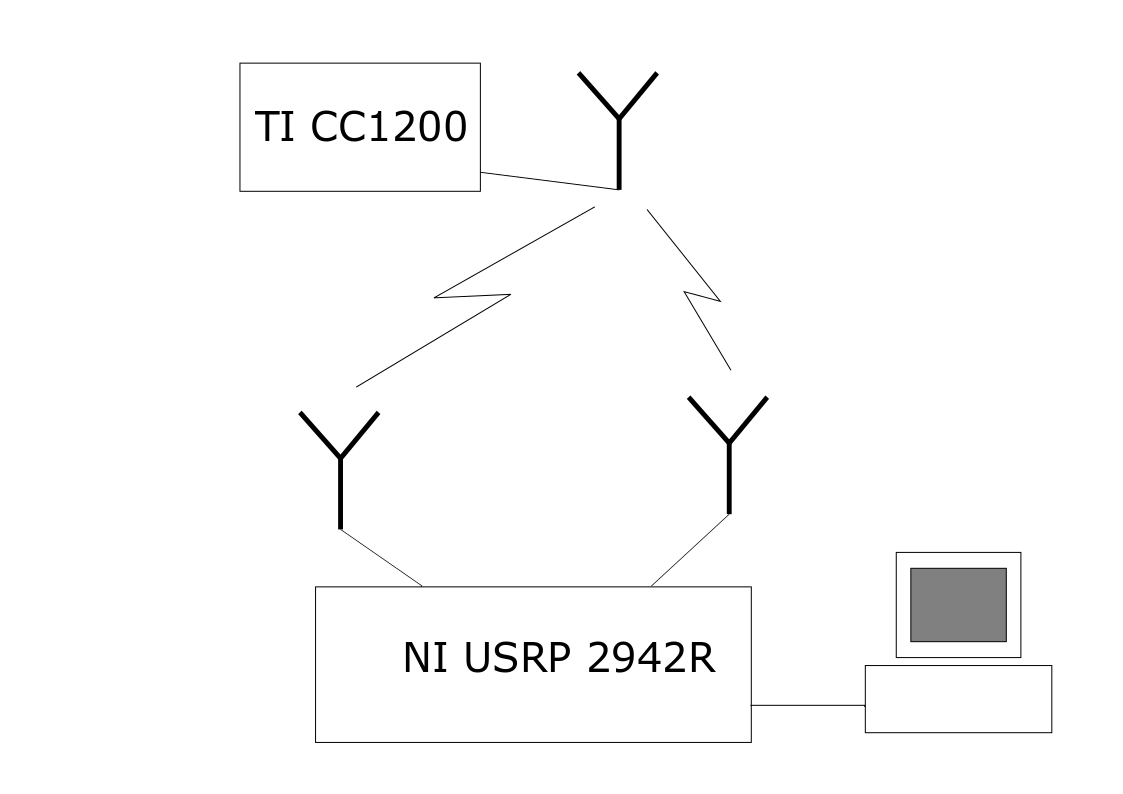
\includegraphics[width=0.7\textwidth]{pics/systemstructure.png}
    \caption{Общая схема предложенной системы}
    \label{fig:SystStructure}
\end{figure}

Измерения производились при расположении узла в трех точках. Здание - железобетонное офисно-промышленное.
План этажа и места расположения элементов экспериментальной установки приведены на Рис.\ref{fig:StagePlan}:
 
\begin{figure}[!htb]
    \centering
    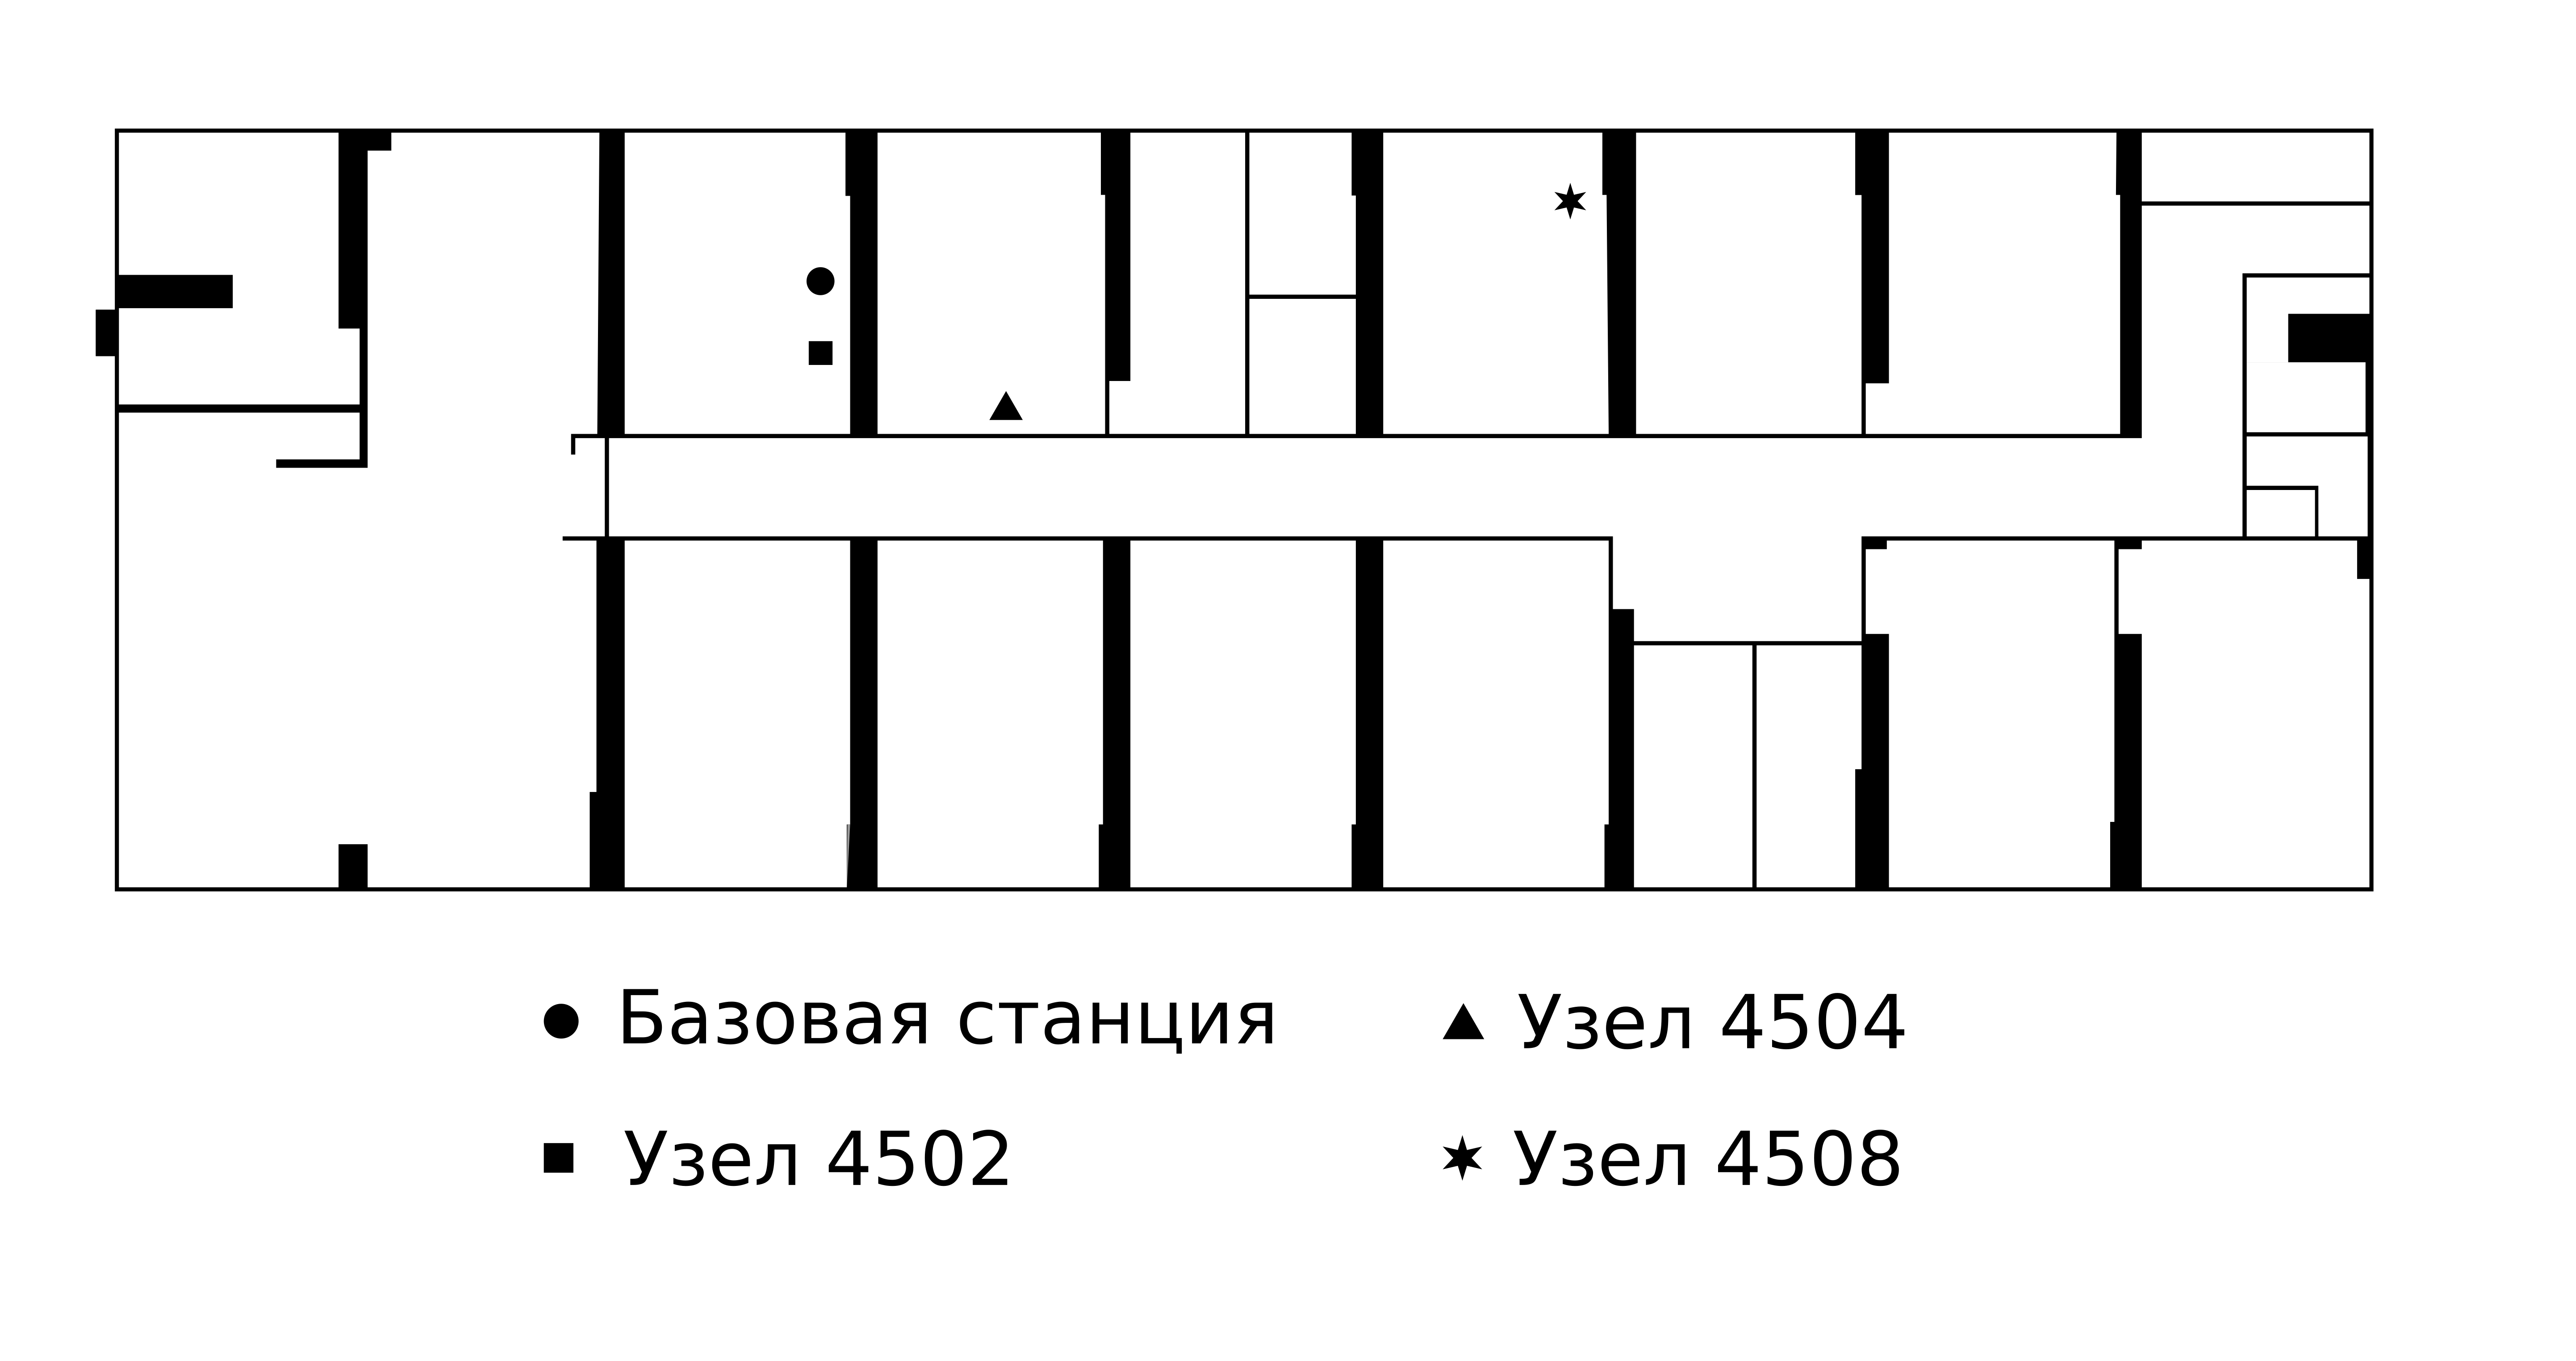
\includegraphics[width=0.9\textwidth]{pics/plan.png}
    \caption{Расположение базовой станции и узлов}
    \label{fig:StagePlan}
\end{figure}

\subsection{Узел}

В качестве сенсора использовался трансивер Texas Instruments CC1200. 
Управление осуществлялось с ПК с помощью ПО SmartRF Studio. 
Настройки приемопередатчика:

\begin{table}[htb!]
\centering
\caption{Настройки радиоканала}
\label{table:ccconfig}
\begin{tabular}{|c|c|}
\hline
Частота несущей & 863 МГц \\
\hline
Скорость передачи & 1 Кбит/c \\
\hline
Модуляция & 2-FSK\\
\hline
Частотная девиация & 9.9945 кГц\\
\hline
\end{tabular}
\end{table}

\subsection{Базовые станции}

В качестве базовых станций использовалось программно-определяемое радиоустройство NI USRP-2942R. Устройство обладает двумя раздельными каналами приема/передачи и таким образом имитирует две базовых станции. 
После аналоговой обработки, оцифрования и опциональной обработки на встроенной ПЛИС принятые сигналы передаются на ПК, где происходят дальнейшие манипуляции по алгоритмам, реализованным в среде LabVIEW. 
При передаче цифровые данные передаются с ПК на USRP, проходят через ПЛИС, ЦАП и переносятся на частоту. 
Блок-схема устройства изображена на Рис.\ref{fig:USRPBD}

\begin{figure}[h!]
\center{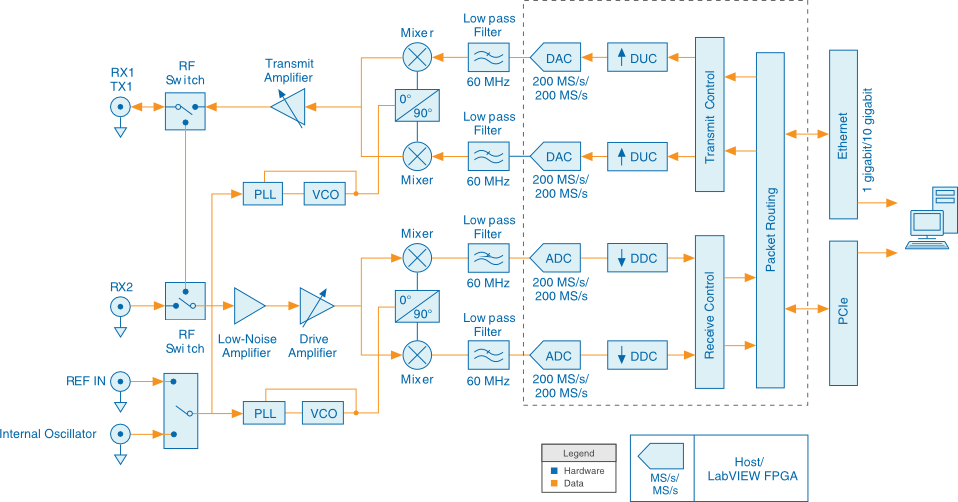
\includegraphics[width=0.8\linewidth]{pics/USRP2942.png}}
\caption{Блок-диаграмма NI USRP 2942R}
\label{fig:USRPBD}
\end{figure}

\subsection{Метрики}
Для оценки качества приема используются различные метрики.
В случае, если прием ведется базовыми станциями, то первичной метрикой является отношение сигнал-шум, как наиболее репрезентативное.
В случае приема узлом используется RSSI ввиду того, что трансивер, используемый в качестве узла, в явном виде поддерживает только LQI (Link Quality Indicator) и RSSI. 
Хотя первая метрика дает больше информации о качестве сигнала, используется RSSI, так как изменения RSSI эквивалентны изменениям SNR (что позволяет проверить справедливость теоретических соотношений).
В качестве вторичной метрики используется PER (Packet Error Rate - уровень ошибок пакетов). Это количество зависит не только от мощности сигнала, но и от его качества - формы импульсов, наличия различного рода помех и т.д.
\clearpage

\section{Характеристики канала}
Исследуемые алгоритмы объединения сигналов налагают определенные ограничения на параметры канала. 
Как указывалось выше, предполагается, что замирания в канале равномерные медленные, т.е. имеет место (\ref{eq:impulse}). 
\subsection{Многолучевое распространение}
Многолучевое распространение, характерное для каналов внутри зданий, приводит к виду импульсной характеристики, отличной от дельта функции \cite{B2}. 
Это приводит к межсимвольной интерференции, которая неизбежно уменьшает прирост качества.
Кроме того, нарушается (\ref{eq:impulse}), что ограничивает применимость иследуемых методов обработки сигналов.

К счастью, в WSN, как правило, нет необходимости обеспечивать большие скорости передачи данных, что позволяет снизить символьные скорости. 
Это увеличивает чувствительность и уменьшает эффект от межсимвольной интерференции. 
Измерения в \cite{A8}, \cite{A9}, что среднеквадратичная задержка в зданиях имеет порядок сотен нс. 
При символьных скоростях 1-10 кбит/с (и соответственно, $T_s = 100-1000$мкс) замирания можно считать частотно-неселективными.

\subsection{Временная зависимость}

Кроме того, реальные каналы не являются статичными; как правило, речь идет о времени, в течении которого характеристики можно считать близкими. 
Изменения канала во времени представляют из себя проблему, так как с течением времени полученные тем или иным образом данные о канале перестают быть актуальными. 
Неверные данные не только ослабляют эффект от применения методов объединения сигналов, но могут и ухудшить ситуацию. 

Как указано выше, скорости в WSN обычно невелики. 
Это приводит к тому, что передача пакета занимает достаточно длительное время. 
При этом канал должен оставаться относительно неизменным в течение времени передачи нескольких пакетов, иначе смысл от использования методов объединения теряется.
Таким образом, возникает необходимость провести исследование канала на статичность.
\subsection{Измерения}
Для того, чтобы узнать, насколько статичен канал, проведен следующий эксперимент. 
Узел передает один и тот же пилот на базовые станции в течение некоторого времени. 
На базовой станции известно содержание пилота, и пакет обнаруживается с помощью кросс-корреляции с принятым сигналом. 
Попутно по максимумам корреляции можно определить и скомпенсировать временные сдвиги между принятыми пакетами. 
Итак,
\begin{equation*}
s_i\left(t\right) = \alpha_i\cdot d\left(t\right)+n\left(n\right),\quad 0\leq t\leq L-1
\end{equation*}

Здесь предполагается, что полезный сигнал уже выделен, и $s_i(t) = 0$ при $t<0$ или $t\geq L$. В реальности там находится шум, но ввиду его малости пренебрежем.

Кросс-корреляция даст:
\begin{gather}
R_i\left(\tau\right) = \sum\limits_{t=-\infty}^{\infty}d^*\left(t\right)s_i\left(t+\tau\right) \approx \nonumber \\ 
\approx \sum\limits_{i=0}^{L-1}\bigl(\alpha_i d^*\left(t\right)d\left(t+\tau\right)+d^*\left(t\right)n\left(t+\tau\right)\bigr) \approx 
\alpha_i\sum\limits_{t=0}^{L-1} d^*\left(t\right)d\left(t+\tau\right) \\
R_i\left(0\right) = \alpha_i\sum\limits_{t=0}^{L-1}|d\left(t\right)|^2 \\
\alpha_i = \frac{R_i\left(0\right)}{\sum\limits_{t=0}^{L-1}|d\left(t\right)|^2}
\label{eq:Crosscor}
\end{gather}

Изменения полученных таким образом комплексных усилений позволят сделать вывод о статичности канала.
\subsection{Результаты}
Замеры (комната 4504) показали, что канал существенно меняется даже на промежутках времени в 1-2 секунды, однако изменение разности фаз между комплексными усилениями остается в пределах на протяжении, к примеру, 20 с. (Рис.\ref{fig:Phases})

В то же время видно, что на больших промежутках времени разность фаз (относительно исходной) может достичь 2 и более. В таком случае при исходной подстройке любой точности мощность принятого сигнала может падать сколь угодно сильно. 
Поэтому в случае более нестационарного канала или большой длительности сессии может возникнуть возможность повторять передачу тренировочных сигналов несколько раз за сессию.

\begin{figure}[!htb]
\begin{minipage}[h]{1\linewidth}
\center{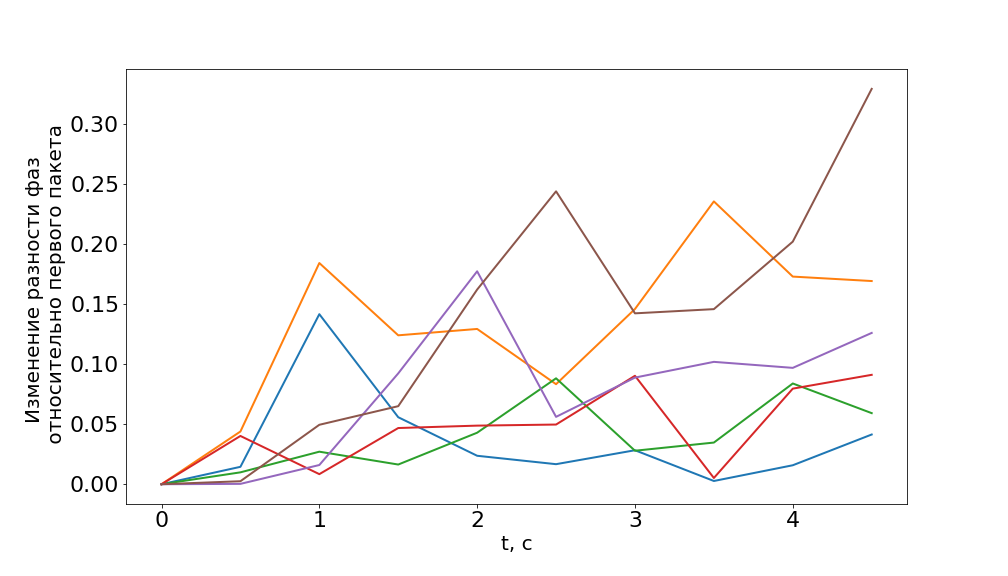
\includegraphics[width=0.8\linewidth]{pics/Phases5.png}} \\
\end{minipage}
\vfill
\begin{minipage}[h]{1\linewidth}
\center{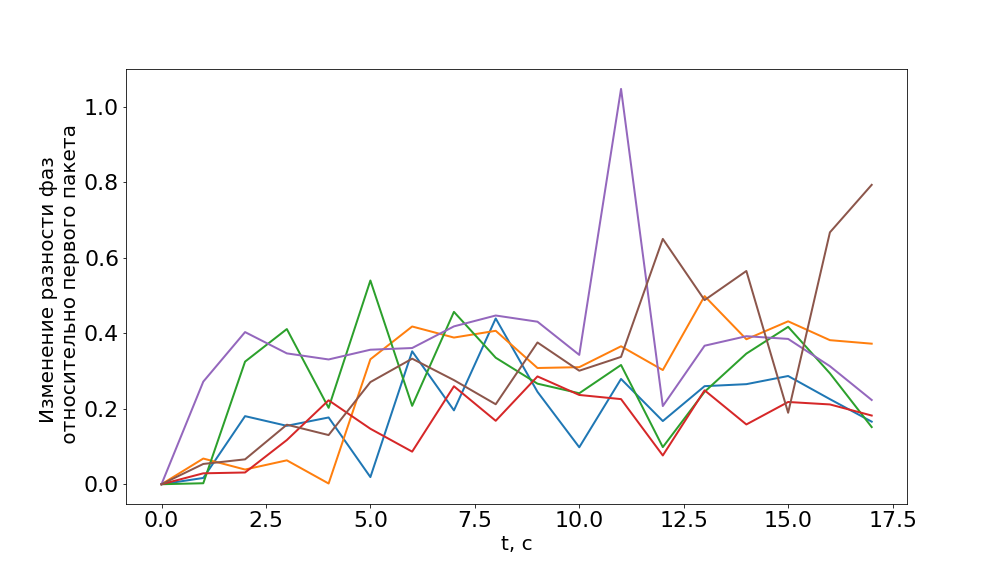
\includegraphics[width=0.8\linewidth]{pics/Phases20.png}} \\
\end{minipage}
\vfill
\begin{minipage}[h]{1\linewidth}
\center{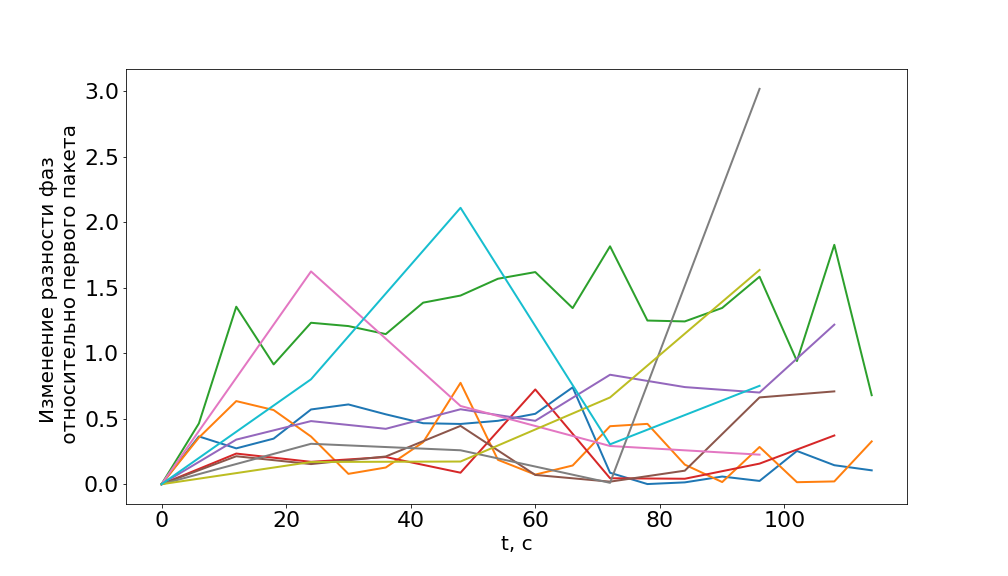
\includegraphics[width=0.8\linewidth]{pics/Phases100.png}} \\
\end{minipage}
\caption{Изменение разности фаз между каналами с течением времени \label{fig:Phases}}
\end{figure}
\FloatBarrier
\section{Восходящая линия связи}

Для проверки производительности EGC и MRC поставлен эксперимент с двумя приемными антеннами; проведены измерения SNR на трех расстояниях для каждого измерения. 
Измерялись отношения сигнал-шум для каждого канала по отдельности и для комбинированного сигнала.

\subsection{Обработка сигналов}

Общая схема обработки принятых сигналов показана на Рис.\ref{fig:SignalProcessing}:

\begin{figure}[!htb]
    \centering
    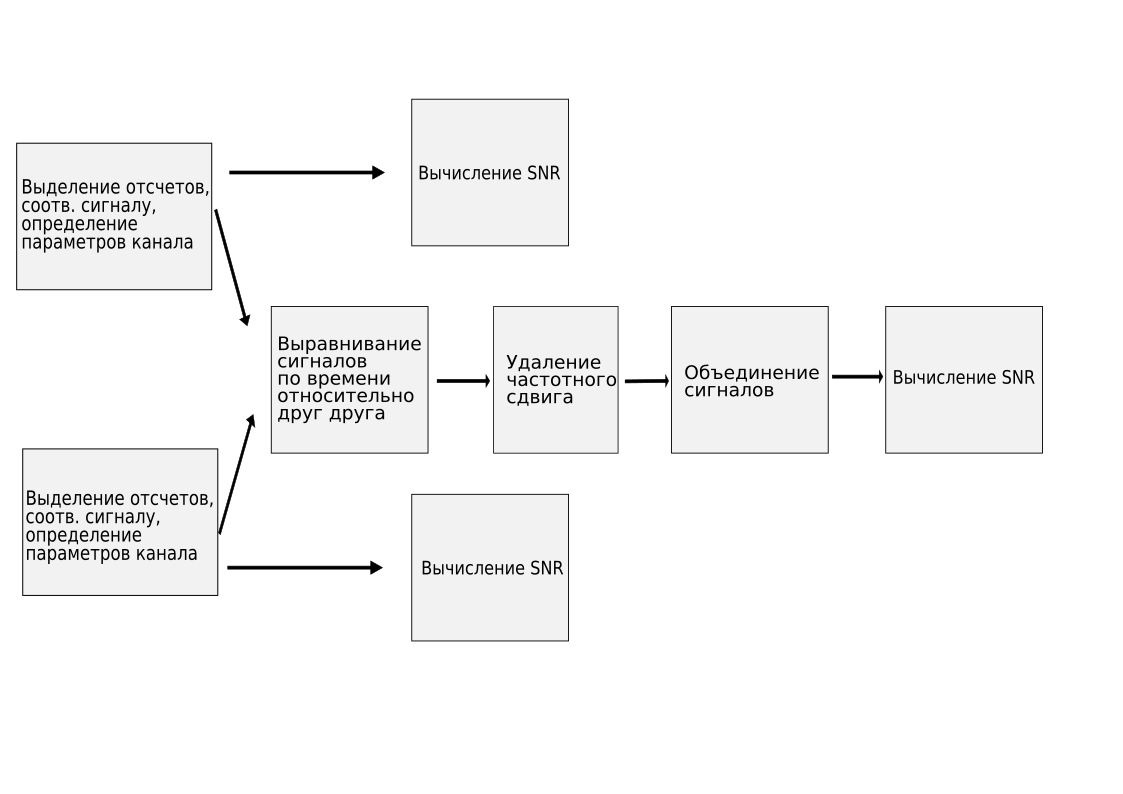
\includegraphics[width=0.9\textwidth]{pics/signalprocessing.png}
    \caption{Схема обработки сигналов}
    \label{fig:SignalProcessing}
\end{figure}

Как и в измерении статичности, пакет обнаруживается с помощью кросс-корреляции пилота с принятым сигналом, и с помощью (\ref{eq:Crosscor}) находится комплексные усиления в каналах. Пакеты выравниваются по времени.
После этого с помощью преобразования Фурье обнаруживается и удаляется остаточный частотный сдвиг - находится положение в спектре середины между тонами, после чего этот частотный сдвиг убирается.

Наконец, происходит объединение сигналов по формулам (\ref{eq:egc}) и (\ref{eq:mrc}). Вычисляется и удаляется разность фаз между сигналами (то же, что и в формулах с точностью до фазового множителя), в MRC идет необходимое домножение по мощности.

\subsection{Результаты эксперимента}

По итогам измерений SNR были построены функции распределения. Их изменение показывает эффективность работы методов \cite{B1}. На графиках видно, что вероятность получить высокое значение отношения сигнал-шум при передаче для фиксированной локации увеличилась:
\begin{figure}[!htb]
\begin{minipage}[h]{0.49\linewidth}
\center{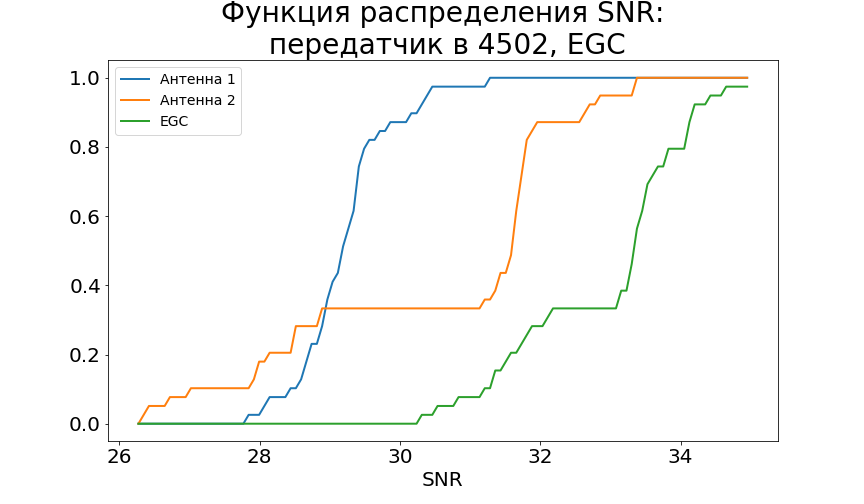
\includegraphics[width=1\linewidth]{pics/midegccdf.png}} \\
\end{minipage}
%/hfill
\begin{minipage}[h]{0.49\linewidth}
\center{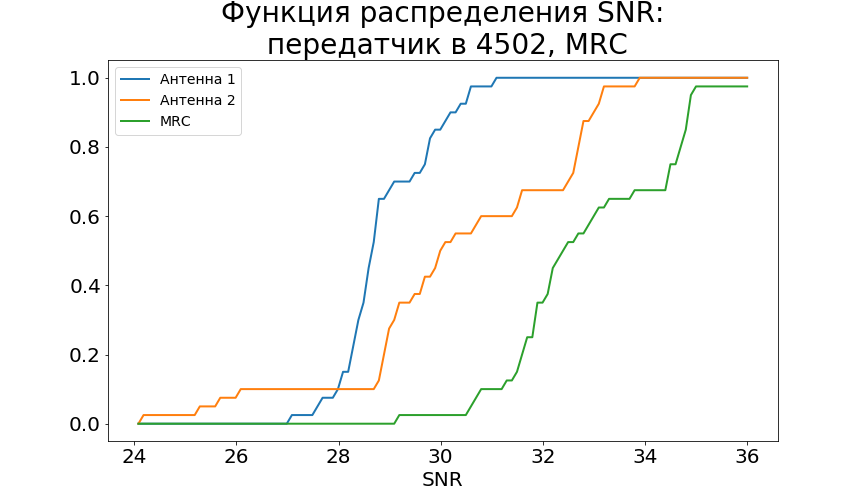
\includegraphics[width=1\linewidth]{pics/midmrccdf.png}} \\
\end{minipage}
\vfill
\begin{minipage}[h]{0.49\linewidth}
\center{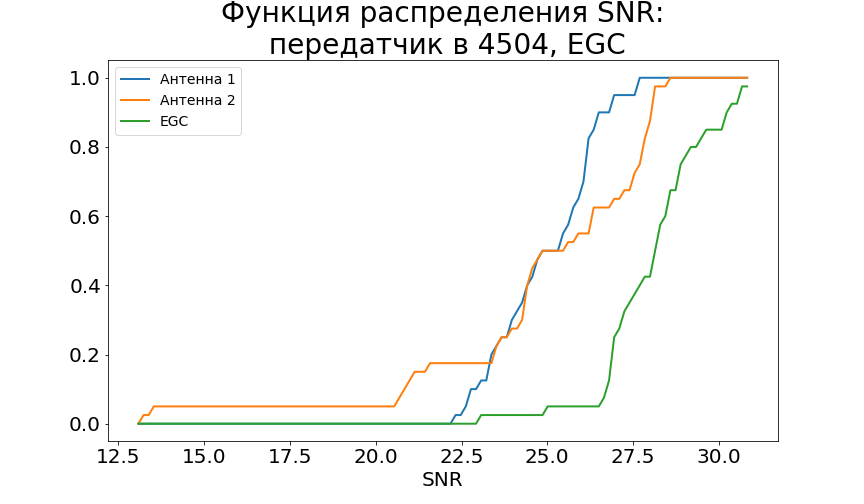
\includegraphics[width=1\linewidth]{pics/neighbegccdf.png}} \\
\end{minipage}
%\hfill
\begin{minipage}[h]{0.49\linewidth}
\center{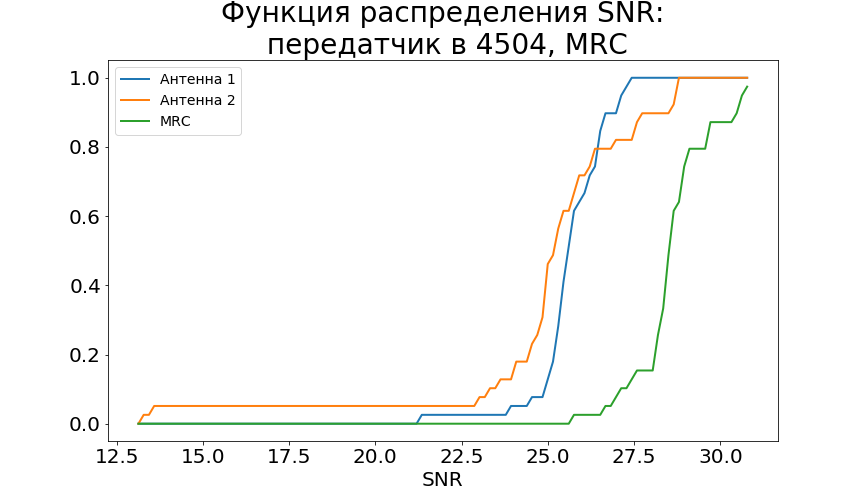
\includegraphics[width=1\linewidth]{pics/neighbmrccdf.png}} \\
\end{minipage}
\vfill
\begin{minipage}[h]{0.49\linewidth}
\center{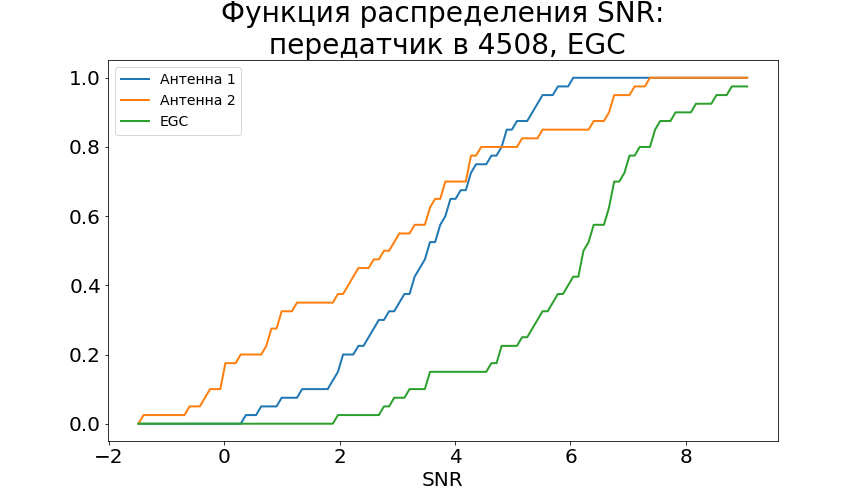
\includegraphics[width=1\linewidth]{pics/longegccdf.png}} \\
\end{minipage}
%\hfill
\begin{minipage}[h]{0.49\linewidth}
\center{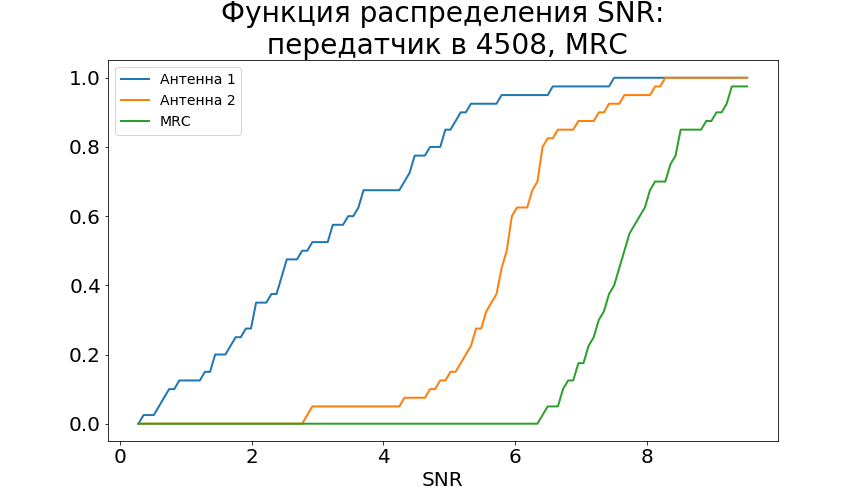
\includegraphics[width=1\linewidth]{pics/longmrccdf.png}} \\
\end{minipage}
\caption{Функции распределения отношения сигнал-шум}
\label{fig:cdfs}
\end{figure}

Можно заметить, что прибавка к SNR в децибелах зависит от баланса SNR в каналах (Рис.\ref{fig:snrbalance}). 
При этом для MRC падение производительности меньше; тем не менее при дисбалансе порядка 6 dB прибавка к итоговому SNR оказывается порядка 1 dB. 
В целом, теоретически ожидаемые значения сигнал-шум слабо отличаются от полученных в эксперименте.
Это показывает Рис.\ref{fig:SNRtheory}. 
Для дальнего расположения передатчика при малых значениях его увеличение несколько ниже теоретического - сказываются сложности с определением параметров канала для слабого сигнала: 

\begin{figure}[h!]
\center{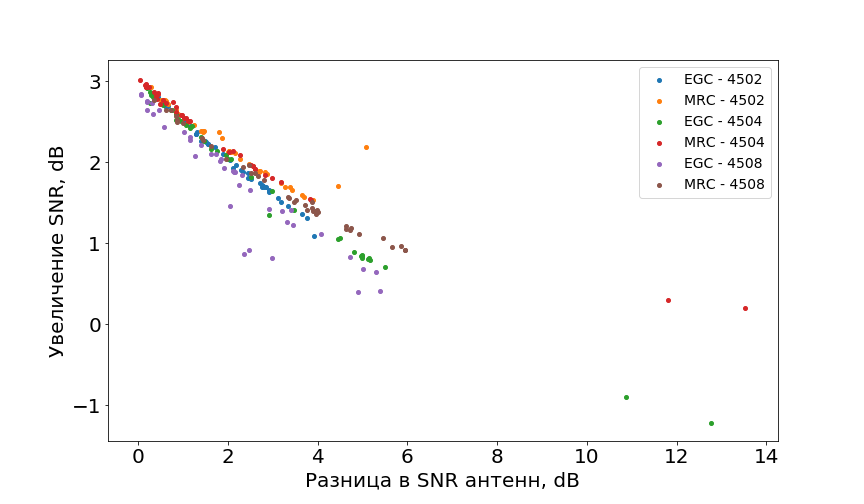
\includegraphics[width=0.8\linewidth]{pics/SNRdiffsnotitle.png}}
\caption{Зависимость увеличения SNR от дисбаланса каналов}
\label{fig:snrbalance}
\end{figure}

\begin{figure}[!htb]
\begin{minipage}[h]{1\linewidth}
\center{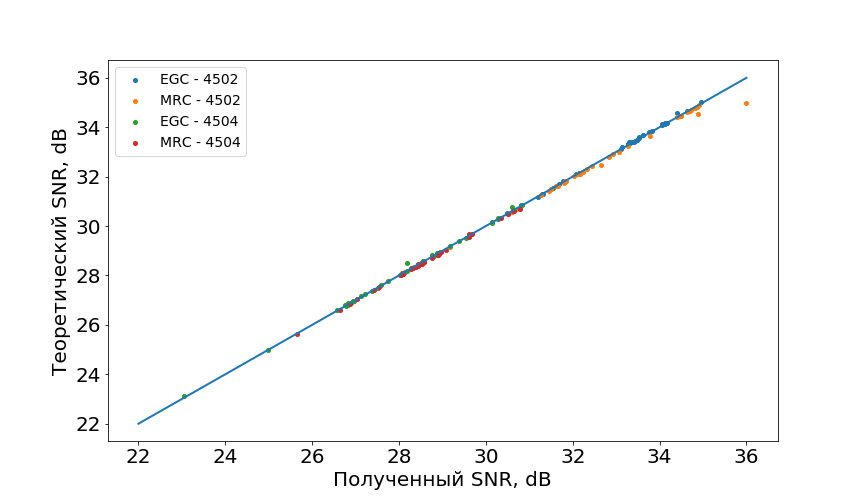
\includegraphics[width=0.8\linewidth]{pics/SNRtheory1notitle.png}} \\
\end{minipage}
\vfill
\begin{minipage}[h]{1\linewidth}
\center{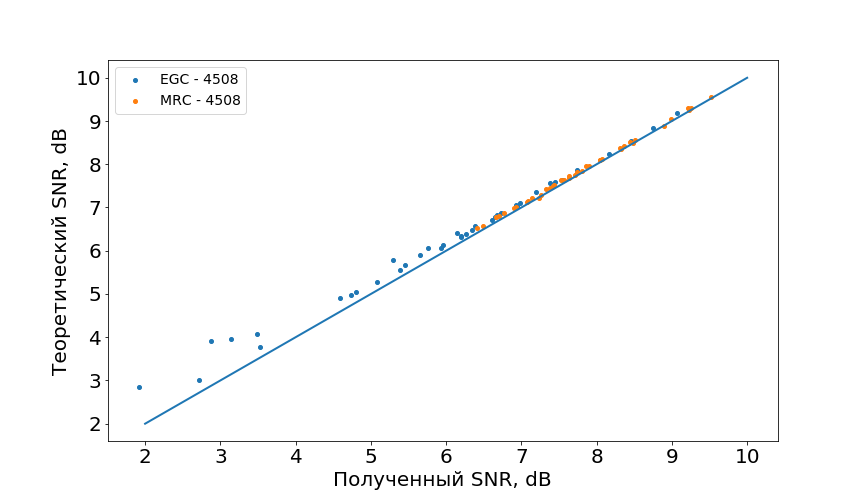
\includegraphics[width=0.8\linewidth]{pics/SNRtheory2notitle.png}} \\
\end{minipage}
\caption{Соответствие теоретического результата и полученного на практике}
\label{fig:SNRtheory}
\end{figure}

\clearpage
\section{Нисходящая линия связи}

Напомним, для передачи с единичным усилением согласно (\ref{eq:egtsignal}):
\begin{equation}
s\left(t\right)=\sum\limits_{i=1}^N \alpha_i\frac{\alpha^*_i}{|\alpha_i|}d\left(t\right) + n\left(t\right) = \left(\sum\limits_{i=1}^N |\alpha_i|\right)d\left(t\right) + n\left(t\right)
\end{equation}
В таком случае SNR имеет следующий вид:
\begin{equation}
\Gamma = \left(\sum\limits_{i=1}^{N}\sqrt{\Gamma_i}\right)^2
\end{equation}
При этом в случае равных усилений в каналах (и, соответственно, равных SNR) получаем 
\begin{equation}
\label{eq:equalSNR}
\Gamma = N^2\Gamma_0
\end{equation}
Для сравнения, MRC и EGC давали меньшее улучшение сигнала:
\begin{equation}
\label{eq:equalSNRMRC}
\Gamma = N\Gamma_0
\end{equation}

\subsection{Стационарность канала}
С одной стороны, метод передачи с единичными усилениями требует относительной стационарности канала на время порядка всей сессии обмена данными между базой и узлом: измерение канала тратит время и заряд, занимает канал. 
По этой причине требуется, чтобы полученные с помощью пилотов характеристики каналов оставались актуальными как можно дольше.

С другой стороны, более высокая производительность (\ref{eq:equalSNR}), (\ref{eq:equalSNRMRC}) позволяет допустить больший разбег по фазам у сигналов, пришедших на принимающую антенну. 
Зависимость усиления от разности фаз показана на Рис.\ref{fig:PDtheory} (для N=2):
\begin{figure}[!htb]
\center{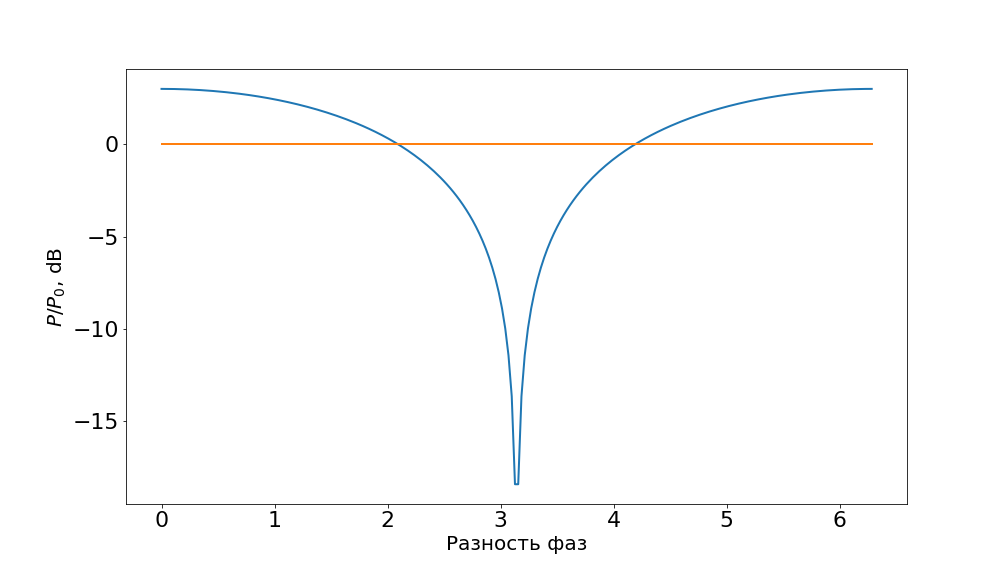
\includegraphics[width=0.8\linewidth]{pics/MRTPDtheory.png}}
\caption{Зависимость усиления от разности фаз между сигналами}
\label{fig:PDtheory}
\end{figure}

Видно, что при лишь разности фаз, большей чем $\Delta\phi=\frac{2\pi}{3}$ усиление обращается в 0 dB. 
При большем числе антенн вероятность получить низкий уровень сигнала из-за деструктивной интерференции уменьшается. 
Тем не менее, эксперимент на стационарность канала показал, что через достаточно долгое время сигналы могут попасть в ситуацию, когда они взаимно уничтожают друг друга, при сколь угодно точной начальной подстройке.

\subsection{Данные о канале}

Метод предполагает известность характеристик каналов. 
Поскольку обработка данных производится до их передачи, передатчики должны заранее получить эти характеристики. 
Пилотные сигналы, передаваемые обычным образом на узлы, плохо подходят ввиду того, что для выяснения характеристик канала к одной базовой станции должны быть проведены следующие действия:
\begin{enumerate}
\item Базовая станция передает сигнал
\item Узел принимает и обрабатывает пилот, извлекая характеристики
\item Узел пересылает данные базовой станции
\end{enumerate}
Поскольку вышеуказанные действия нужно производить последовательно, то от узла требуется принять, обработать и послать обратно порядка N пакетов, что негативно скажется на его времени работы. 
Кроме того, процедура измерения канала требует много времени (особенно с учетом вычислительных мощностей узла), ввиду чего усугубляются проблемы с нестационарностью канала.

Есть и другой подход - использование принципа взаимности. 
В таком случае узел рассылает один пилот, и для каждой антенны получается характеристика канала "узел - базовая станция". 
Эти характеристики используются для передачи в обратную сторону. 
С одной стороны, этот метод проще в реализации, экономичнее расходует канал и гораздо меньше нагружает узел. 
Проблема заключается в том, что принцип взаимности должен выполнятся не для радиочастотного канала в одиночку, а для его совокупности с выходным трактом передатчика, начиная с миксеров. 
В большей части реализаций приемопередатчиков на приеме и передаче стоят различные синтезаторы частоты, разность фаз между которыми никак не зафиксирована. 
По этой причине разности фаз между комплексными усилениями каналов случайным образом отличаются от измеренных, что делает метод бессмысленным либо вынуждает строить систему со сложным и дорогим оборудованием синхронизации.

В качестве решения проблемы предлагается отказаться от точной подстройки фазы. Рассмотрим два варианта такого рода действий:

Суть первого метода заключается в попытке оценить разности фаз между комплексными усилениями каналов некоторым дискретным набором значений. 
В таком случае базовые станции по очереди подстраиваются к одной - ведущей - путем передачи k тренировочных пакетов, где между i-ыми сигналами с антенн внесена разность фаз $\frac{2*\pi*(i-1)}{k}$. 
Узел замеряет мощность принятых сигналов, и в обратном пакете сообщает о варианте, давшем лучший результат. 
Выбор самого сильного сигнала позволяет узнать разность фаз между комплексными усилениями каналов с точностью $\pm\frac{\pi}{k}$. 
В таком случае среднее усиление сигнала на узле:
\begin{gather}
\frac{P}{P_0} = \left(\frac{k}{2\pi}\right)^N\int\limits_{-\frac{\pi}{k}}^{\frac{\pi}{k}}\ldots\int\limits_{-\frac{\pi}{k}}^{\frac{\pi}{k}}\bigl|1+e^{i\Delta\varphi_1}+\ldots+e^{i\Delta\varphi_{N-1}}\bigr|^2d\Delta\varphi_1\ldots d\Delta\varphi_{N-1} = \nonumber \\
= N + \sum\limits_{i\neq j}\left(\frac{k}{2\pi}\right)^2\int\limits_{-\frac{\pi}{k}}^{\frac{\pi}{k}} e^{i\Delta\varphi_i} d\Delta\varphi_i \int\limits_{-\frac{\pi}{k}}^{\frac{\pi}{k}} e^{-i\Delta\varphi_j}d\Delta\varphi_j + \sum\limits_{i}\frac{k}{2\pi}\int\limits_{-\frac{\pi}{k}}^{\frac{\pi}{k}} \left( e^{i\Delta\varphi_i} + e^{-i\Delta\varphi_i}\right)d\Delta\varphi_i = \nonumber \\
= N +  \sum\limits_{i\neq j}\left(\frac{k}{2\pi}\right)^2\frac{e^{i\frac{\pi}{k}}-e^{-i\frac{\pi}{k}}}{i}\frac{e^{-i\frac{\pi}{k}}-e^{i\frac{\pi}{k}}}{-i}+\sum\limits_{i}\frac{k}{2\pi}\left(\frac{e^{i\frac{\pi}{k}}-e^{-i\frac{\pi}{k}}}{i}+\frac{e^{-i\frac{\pi}{k}}-e^{i\frac{\pi}{k}}}{-i}\right) = \nonumber \\
= N + \left(N-1\right)\left(N-2\right)\left(\frac{k}{\pi}\right)^2sin^2\left(\frac{\pi}{k}\right)+2\left(N-1\right)\frac{k}{\pi}sin\left(\frac{\pi}{k}\right) < N^2
\end{gather}
Этот метод слабо нагружает узел, а также позволяет обойти проблему с принципом взаимности. 
%Видно, что количество антенн линейно увеличивает количество пилотных сигналов. Это может быть проблемой при больших N, т.к пилотные сигналы занимают канал; компромисс между точностью подстройки и увеличением качества приема рассматривается ниже.

Другой подход предполагает вовсе отказаться от пилотных сигналов и не обращать никакого внимания на фазы. В случае такой некогерентной передачи сигналы складываются по мощности:
\begin{gather}
\Gamma = \frac{1}{\left(2\pi\right)^N}\iint\bigl|\sum\limits_{i=1}^Ne^{i\varphi_i}\bigr|^2d\varphi_1\ldots d\varphi_N = N + \sum\limits_{i\neq j}\frac{1}{\left(2\pi\right)^2}\int e^{i\varphi_i} d\varphi_i \int\limits e^{-i\varphi_j}d\varphi_j = N
\end{gather}

В данном случае, в работу узла вовсе не предполагается вносить каких-либо изменений по сравнению с SISO. Тем не менее, несмотря на кажущуюся простоту некогеретной передачи, даже у ее реализации есть нюансы, на которые необходимо обратить внимание.

\subsection{Проблемы имплементации}

Некоторые из имеющихся проблем с имплементацией специфичны для того или иного метода, а некоторые характерны для методов, использующих сложение на антенне узла в целом:
\begin{enumerate}
\item Как уже было замечено, канал меняется не очень быстро.
В случае неудачного сочетания фаз при отказе от пилотов система рискует попасть в "ущелье" на Рис.\ref{fig:PDtheory} и оставаться в нем в течение достаточно долгого времени. 
Эта проблема решается внедрением меняющейся разности фаз (линейно или же случайно).
В таком случае неудовлетворительная разность фаз в случае возникновения долго не задержится.

\item В случае метода, использующего оценку разности фаз конечным набором значений, приходится идти на компромисс между точностью подстройки и ростом нагруженности канала. Если пилотов будет слишком много, то может быть превышена емкость канала.

Рассмотрим конфигурацию, в которой на одно измерение приходятся L пакетов полезной нагрузки фиксированного размера (136 байт). 
Пусть передано k пилотов. 
Тогда реальную разность фаз можно считать равномерно распределенной по интервалу $\left[0, \frac{\pi}{k}\right]$ (знак неважен). 
Используется FSK, поэтому вероятность ошибки в бите при заданном SNR задается \cite{B2}:

\begin{equation}
P_{b-fixed} = \frac{1}{2}exp\left(-\frac{1}{2}\frac{E_b}{N_0})\right)
\label{eq:FSKBER}
\end{equation}
Тогда посчитаем полную вероятность ошибки в бите:
\begin{equation}
\begin{gathered}
P_b = \frac{k}{\pi}\int\limits_0^\frac{\pi}{k}\frac{1}{2}exp(-\frac{1}{2}\frac{E_b}{N_0}(2+2cos\phi))d\phi = \frac{k}{2\pi}exp(-\frac{E_b}{N_0})\int\limits_0^\frac{\pi}{k}e^{-\frac{E_b}{N_0}cos\phi}d\phi \leq \\
\leq \frac{k}{2\pi}exp(-\frac{E_b}{N_0})\int\limits_0^\frac{\pi}{k}e^{-\frac{E_b}{N_0}cos\frac{\pi}{k}}d\phi = \frac{1}{2}e^{-\frac{E_b}{N_0}(1+cos(\frac{\pi}{k}))}
\end{gathered}
\label{eq:FullBER}
\end{equation}

Результат иллюстрирует Рис.\ref{fig:ErrorProbPlane}. Видно, что по мере увеличения числа пакетов эффект падает, поэтому передача большого количества тренировочных пакетов может быть нерациональной.

\begin{figure}[!htb]
\center{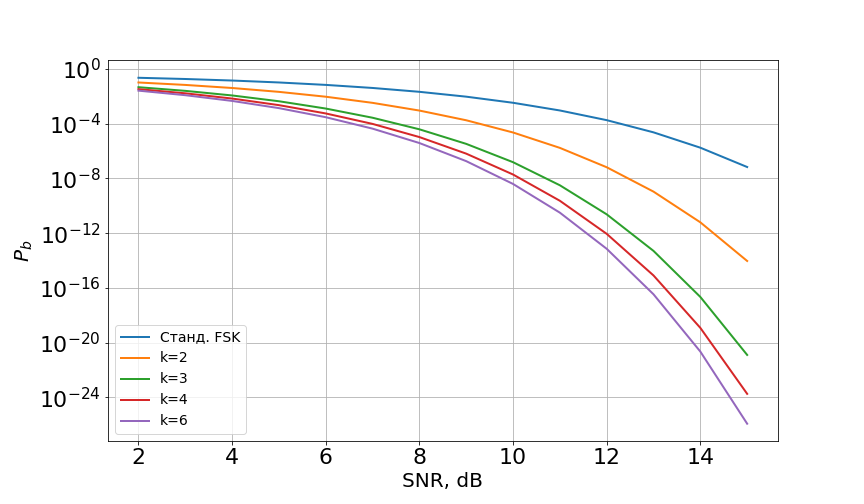
\includegraphics[width=0.8\linewidth]{pics/ErrorProbPlane.png}}
\caption{Зависимость вероятности ошибки в бите от отношения сигнал-шум при разных k}
\label{fig:ErrorProbPlane}
\end{figure}
\FloatBarrier
При этом увеличение траффика вычисляется по простой формуле:
\begin{equation}
\frac{\Delta Tr}{Tr} = \frac{k}{L} * 100\%
\label{eq:Traffic}
\end{equation}

\item В отличие от восходящей линии связи, в данном случае требуется достаточно хорошая синхронизация между базовыми станциями по частоте и времени. 
\begin{enumerate}
\item Рассинхронизация по частоте будет приводить к набегу с течением времени дополнительной разности фаз, из-за чего производительность при любой стратегии работы с разностями фаз падает до произодительности некогеретной передачи.
В случае особенно больших разностей частот несущих могут наблюдаться сбои в работе демодулятора узла.
В таком случае система может стать неработоспособной.

\item Временная рассинхронизация приводит к возникновению межсимвольных помех. 
Для обычного многолучевого распространения задержанные сигналы, как правило, достаточно быстро убывают с течением времени. 
В данном случае, если сигналы, пришедшие от базовых станций, имеют близкие мощности (в этом случае, кстати, при идеальной синхронизации методы работают лучше всего), то полученные межсимвольные помехи могут привести к неспособности узла демодулировать полученный сигнал.
Результаты симуляции уровня битовых ошибок показаны на Рис.\ref{fig:BERtiming}:

\begin{figure}[!h]
\center{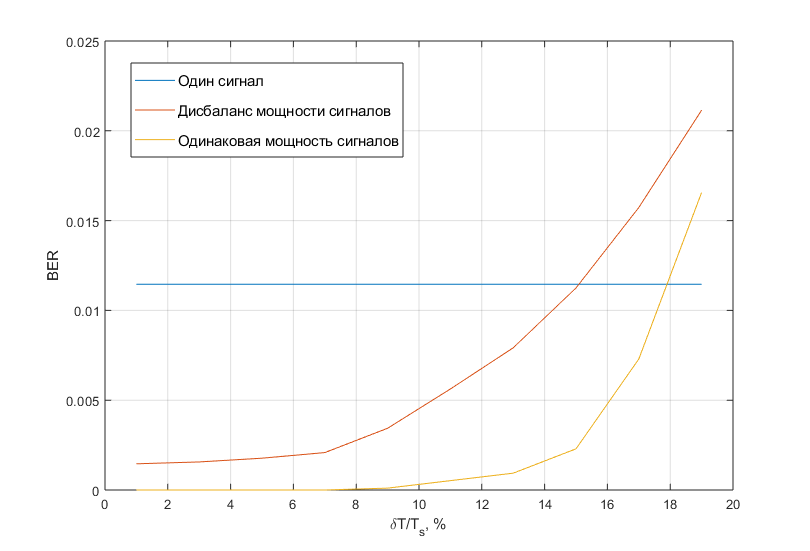
\includegraphics[width=0.8\linewidth]{pics/modesnotitle.png}}
\caption{Зависимость BER от временной синхронизации}
\label{fig:BERtiming}
\end{figure}
\FloatBarrier
Так как \mbox{$PER = 1-\left(1-BER\right)^l\propto l\cdot BER$}, поведение PER ожидается аналогичным.
\end{enumerate}
\end{enumerate}

\subsection{Эксперимент}
\subsubsection{Мощность сигнала}
Для того, чтобы проверить на практике работоспособность вышеописанных методов, проведены наблюдения изменения мощности сигнала при переборе разности фаз.

При проверке работы Phase Sweeping данные передавались с базы на узел, где замерялся RSSI. 

%\begin{figure}[h!]
%\center{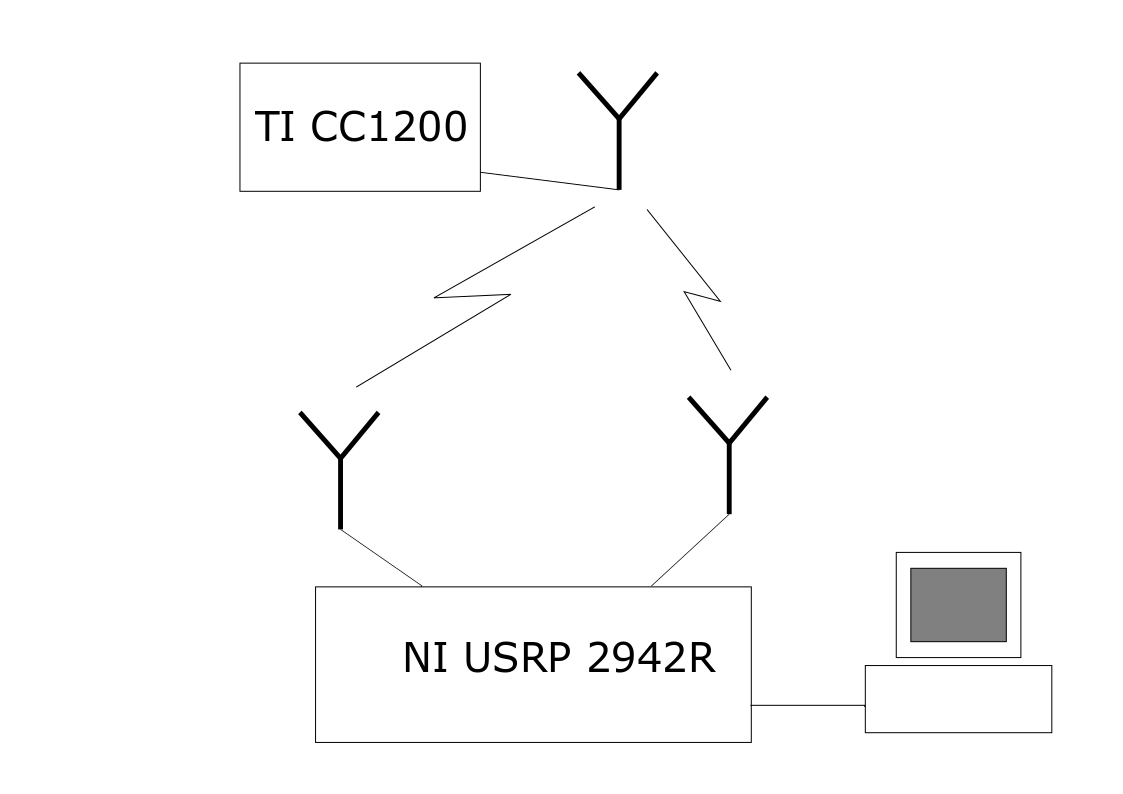
\includegraphics[width=0.5\linewidth]{pics/systemstructure.png}}
%\caption{Структура экспериментальной системы}
%\label{syststruct2}
%\end{figure}

На Рис.\ref{fig:4508} показаны результаты 12 испытаний. 
Сначала передавались 40 пакетов с изменяющейся разностью фаз (синий график), после чего 5 пакетов с одной антенны (оранжевая линия - среднее значение). 
Результаты измерений RSSI отложены по оси ординат. 
Видно, что картина очень похожа на теоретическую; также можно отметить существенную прибавку по мощности относительно передачи с одной антенны.
\begin{figure}[H]
\center{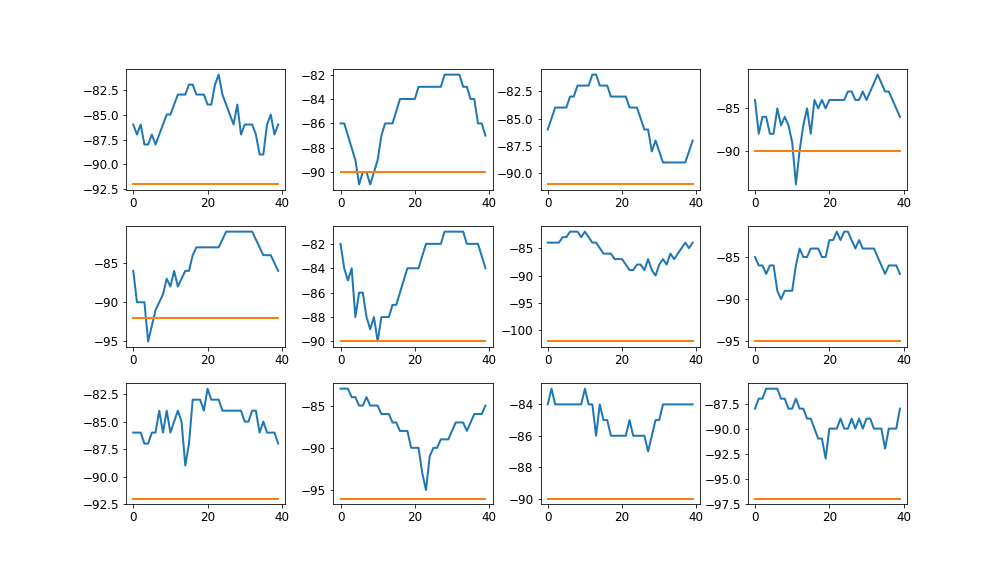
\includegraphics[width=0.9\linewidth]{pics/Phasesweep.png}}
\caption{Результаты измерений RSSI при Phase Sweeping, комната 4508}
\label{fig:4508}
\end{figure}

Так как все методы отличаются лишь выбором начальной разности фаз ("точная" оценка, ближайшая оценка из конечного набора, случайная), то результаты применимы к ним всем. Отличие заключается лишь в том, в какой части графика будет система будет находиться изначально.
В рассматриваемой конфигурации в сеансе связи обычно используются 22 пакета (иногда больше). 
Посчитаем, как вырастет использование канала при 1 измерении на 22 пакета, и соответствие уменьшения ошибки этому росту, исходя из (\ref{eq:FullBER}) и (\ref{eq:Traffic}). 
График можно увидеть на Рис.\ref{fig:BERvsChannel}. Видно, что передавать чересчур много пилотов нерационально - падение уровня ошибок замедляется.

\begin{figure}[h!]
\center{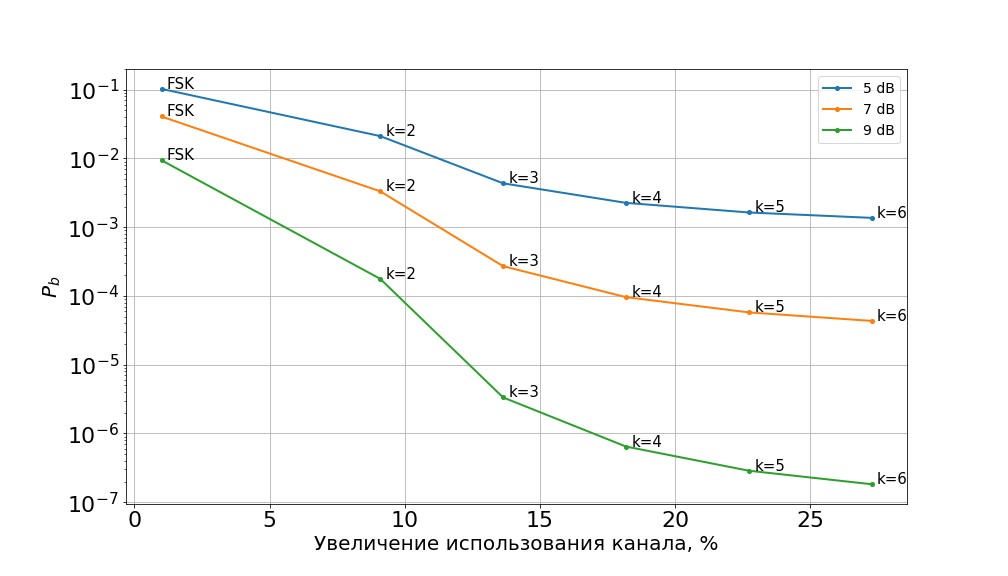
\includegraphics[width=0.8\linewidth]{pics/BERvsChannel.png}}
\caption{Вероятность ошибки в бите и использование канала при разном числе тренировочных пакетов при Phase Sweeping}
\label{fig:BERvsChannel}
\end{figure}

\subsubsection{Качество демодулирования}
Для исследования влияния временной рассинхронизации на прием пакетов также был поставлен эксперимент. 
С базовых станций на узел передавались пакеты с разной временной задержкой. 
Поскольку RSSI в таком случае не является информативным, используется PER.
Использовалась некогерентная передача с внесением случайной фазы и без него, с дисбалансом каналов по мощности и при сравнимых мощностях сигналов на антенне узла. 
При проведении измерений с помощью умножения передаваемых данных на изменяемый множитель изменялась мощность сигнала на антенне узла.
Таким образом удалось получить данные о поведении метода при разных мощностях.

На больших мощностях поведение уровня ошибок в зависимости от рассинхронизации пакетов совпадет с теоретическим (Рис.\ref{fig:Timing40}).

\begin{figure}[!htb]
\center{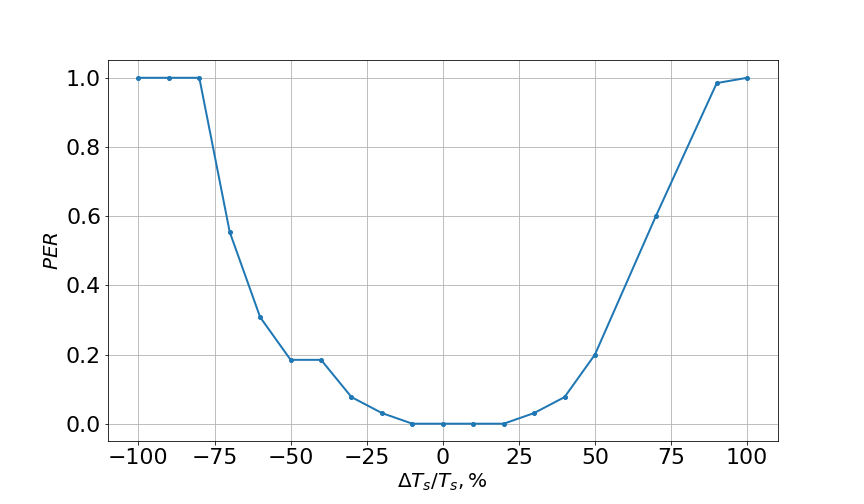
\includegraphics[width=0.8\linewidth]{pics/Timing401.png}}
\caption{Уровень ошибок при ослаблении 40 dB}
\label{fig:Timing40}
\end{figure}

Далее, по мере ухудшения качества сигнала из-за затухания, наблюдается следующее явление. 
Сначала приемник перестает справляться с приемом скомбинированного сигнала - возникают большие значения PER даже при наилучшей синхронизации по времени. 
При демодулировании сигнала от одной антенны ошибки также имеются, однако их существенно меньше (Рис.\ref{fig:Timing45}).

\begin{figure}[!htb]
	\center{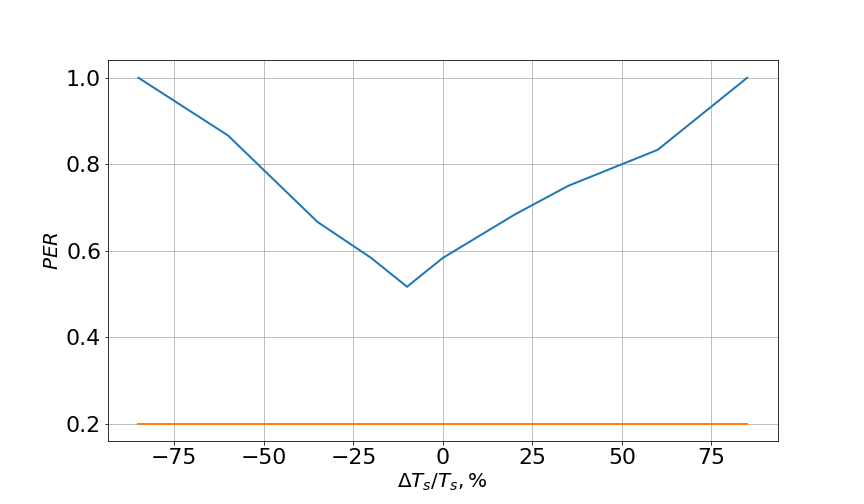
\includegraphics[width=0.8\linewidth]{pics/Timing451.png}}
	\caption{Уровень ошибок при ослаблении 45 dB, с внесением случайной фазы}
	\label{fig:Timing45}
\end{figure}

%\begin{figure}[!htb]
%\center{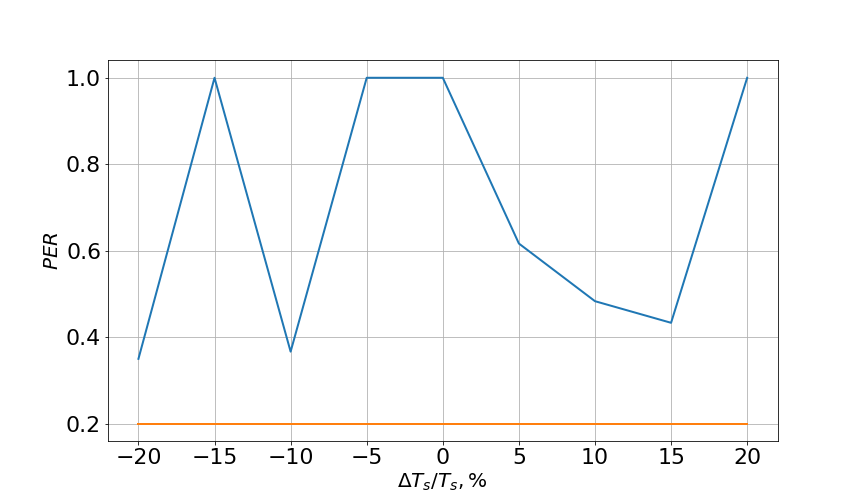
\includegraphics[width=0.8\linewidth]{pics/Timing461.png}}
%\caption{Уровень ошибок при ослаблении 46 dB, без внесения случайной фазы}
%\label{fig:Timing46}
%\end{figure}

\FloatBarrier
Однако, по мере дальнейшего ухудшения сигнала ситуация меняется. 
На Рис.\ref{fig:Timing47} видно, что сигнал от одной антенны становится настолько слабым, что большая часть пакетов не достигает назначения (Фактически, узел просто перестает их обнаруживать - порог обнаружения преамбулы не пройден). 
При этом в случае работы с двух антенн уровень ошибок хотя и оставляет желать лучшего, однако позволяет пересылать хотя бы часть пакетов.
При этом большая часть пакетов успешно обнаруживается, но отбрасывается ввиду ошибок демодулирования и последующего провала проверки CRC.

Рис.\ref{fig:Timing47yes} соответствует передаче с внесением случайной добавки по фазе в передаваемые данные. 
Видно, что в таком случае результаты более стабильны, чем на Рис.\ref{fig:Timing47no}, так как в таком случае попадания в локальные пики замираний (и как следствие, провалы производительности) нивелируются за счет усреднения.
Рис.\ref{fig:Timing47disb} почти не отличается от предыдущего. Единственное, при большой рассинхронизации уровень ошибок растет медленнее - демодулятору проще справиться с более слабой помехой.

\begin{figure}[!h]
	\centering
	\begin{subfigure}[h]{0.7\linewidth}
		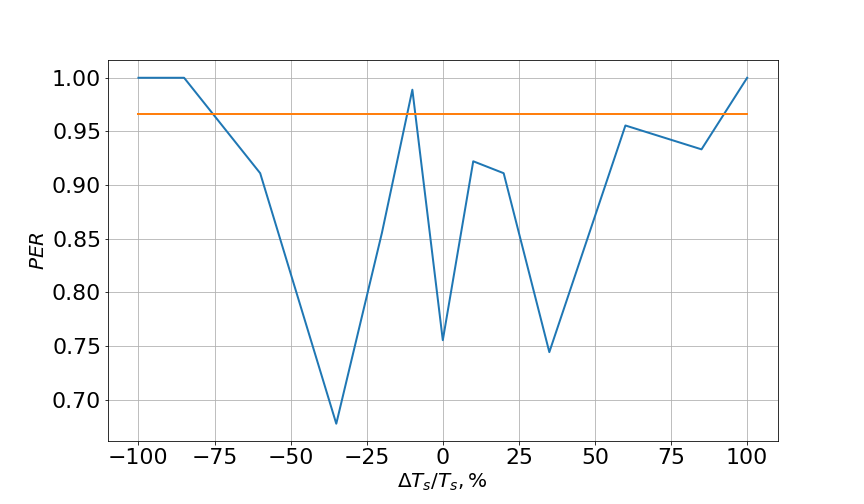
\includegraphics[width=\textwidth]{pics/Timing4711.png}
		\caption{Без внесения случайной фазы}
		\label{fig:Timing47no}
	\end{subfigure}
	\begin{subfigure}[h]{0.7\linewidth}
		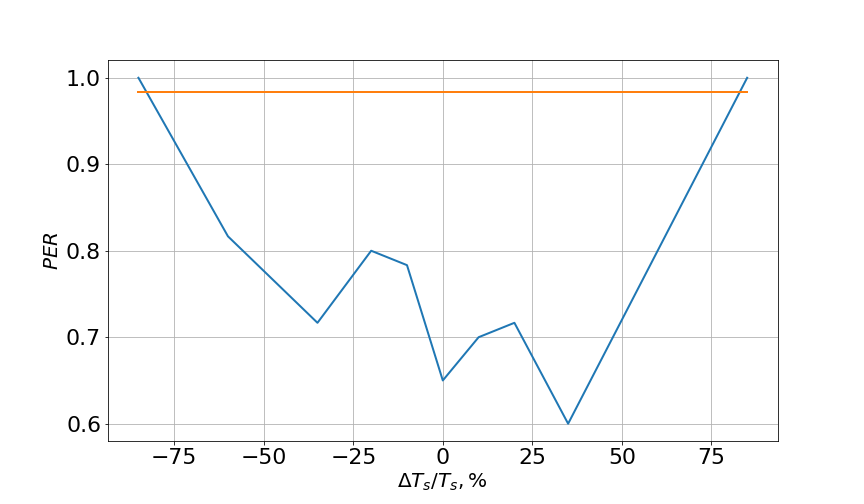
\includegraphics[width=\textwidth]{pics/Timing4721.png}
		\caption{С внесением случайной фазы}
		\label{fig:Timing47yes}
	\end{subfigure}
	\begin{subfigure}[h]{0.7\linewidth}
		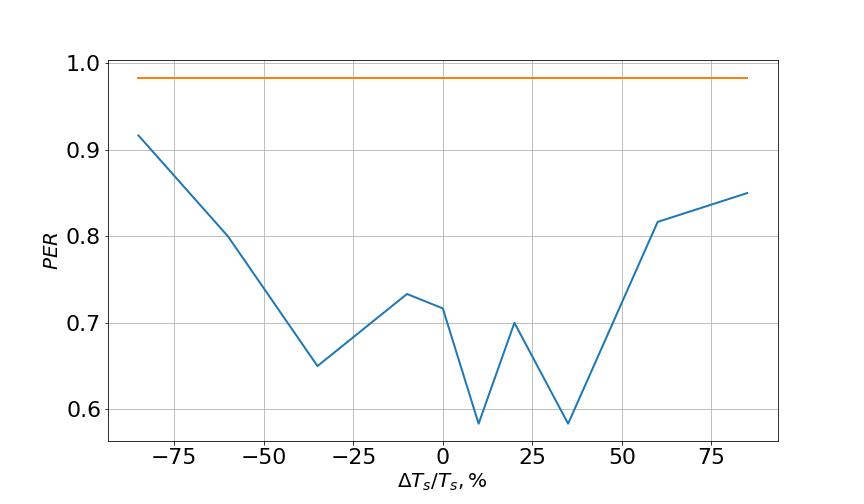
\includegraphics[width=\textwidth]{pics/Timing4731.png}
		\caption{С внесением случайной фазы и дисбалансом каналов $\sim$ 3dB}
		\label{fig:Timing47disb}
	\end{subfigure}
	\caption{Уровень ошибок при ослаблении в 47 dB}
	\label{fig:Timing47}
\end{figure}
\FloatBarrier
\subsubsection{Итоги}

Из результатов видно, что ставка на некогерентную передачу с точки зрения мощности принятого сигнала оправдала себя - в большинстве случаев принятый с двух антенн сигнал был мощнее на несколько децибел.

К сожалению, с точки зрения уровня ошибок результаты оказались менее хорошими.
Эксперимент показал, что штатный демодулятор на узле при приеме с нескольких антенн в большинстве случаев работает хуже, чем при приеме с одной антенны ввиду неизбежного искажения сигнала. 
Тем не менее, в случаях очень слабого сигнала появляется возможность установить хоть какое-то соединение. 
Так как реализация передачи с нескольких антенн не требует существенного изменения системы, то является вполне реалиуемой гибридная система: пока позволяет канал, идет SISO передача, однако как только сигнал проседает ниже уровня приема узлом, происходит переключение на мультиантенный режим.
Кроме того, применение более комплексных решений на узле может нивелировать эффекты наложения сигналов, к примеру, с помощью эквалайзеров\cite{B2}.

Тем не менее, вопросы синхронизации передатчиков по частоте и времени остаются открытыми.

\clearpage

\section{Заключение}

Целью работы был анализ методов объединения пространственно разнесенных сигналов в применении к беспроводной сенсорной сети. 
Помимо теоретической оценки производительности методов, были проведены опыты, целью которых было уточнение требований к инфраструктуре сети и более точного определения эффекта от использования этих методов.

В случае восходящей линии связи были рассмотрены MRC и EGC.
Улучшение SNR, линейное по количеству антенн, подтвердилось; тем не менее, лучшая производительность наблюдается при примерно одинаковых по SNR каналах.
В противном случае производительность падает.
Хотя эти методы требуют модернизацию базовых станций относительно SISO-варианта, факт обработки данных в цифровой области упрощает внедрение метода.

На нисходящей линии связи наблюдается противоположная картина. 
Хотя сложение сигналов на антенне теоретически сулит квадратичное по количеству антенн усиление сигнала, реализация когерентного сложения не представляется разумной.
Даже в случае некогеретного сложения работоспособность системы существенно зависит от синхронизации между базовыми станциями.
Невозможность идеально синхронизировать базовые станции приводит к неустойчивости работы демодулятора; без использования устойчивого демодулятора метод некогеретного сложения может применяться в качестве средства последней надежды на краю области приема, где мощность сигнала экстремально низкая.

Дальнейшие исследования будут посвящены вопросам практической реализации вышеописанных методов. 

\cleardoublepage
\begin{thebibliography}{99}
\bibitem{A1} Dave Evans. The Internet of Things. How the Next Evolution of the Internet Is Changing Everything. Cisco White Paper. Cisco Systems (11 April 2011)
\bibitem{A2} Рекомендация МСЭ-T Y.2069: Термины и определения для интернета вещей 
\bibitem{B1} Andreas F. Molisch, “Wireless Communications” 2nd edition, John Wiley \& Sons, 2011.
\bibitem{A3} Mi-Kyung Oh, Xiaoli Ma, Georgios B. Giannakis, Dong-Jo Park, "Cooperative synchronization and channel estimation in wireless sensor networks", Journal of Communications and Networks, Volume 7, 2005
\bibitem{A4} R.Roy, A.Paulraj and T.Kailath, "Direction-of-Arrival Estimation by Subspace Rotation Methods - ESPRIT", 1986 ICASSP '86. IEEE International Conference on Acoustics, Speech, and Signal Processing
\bibitem{A5} Jia-jia Rong, Feng-gang Yan, Shuai Liu, "Computationally efficient direction of arrival estimation without subspace decomposition", 2016 IEEE 13th International Conference on Signal Processing (ICSP)
\bibitem{A6} R.O.Schmidt, "Multiple emitter location and signal parameter estimation", In Proc. RADC Spectrum Estimation Workshop, pages 243-258, Griffiths AFB , N.Y., 1979
\bibitem{A7} V. Umadevi, P. Easwaran, "A Study on Rake Receivers",  2017 IEEE International Conference on Electrical, Instrumentation and Communication Engineering (ICEICE)
\bibitem{B2} Bernard Sklar, "Digital Communications: Fundamentals and Applications", 2nd Edition, Prentice Hall P T R, 2001
\bibitem{A8} D.M.J. Devasirvatham, R.R. Murray, C. Banerjee, "Time delay spread measurements at 850 MHz and 1.7 GHz inside a metropolitan office building", Electronics Letters, 1989
\bibitem{A9} D.M.J. Devasirvatham, "Time delay spread and signal level measurements of 850 MHz radio waves in building environments", IEEE Transactions on Antennas and Propagation, 1986
\end{thebibliography}

\addcontentsline{toc}{section}{Список литературы}
%=====================================================
\cleardoublepage

\end{document}

